\documentclass[oneside]{scrreprt}
\usepackage[polish]{babel}
\usepackage[utf8]{inputenc}
\usepackage{listings}
\usepackage{graphicx}
\usepackage{aeguill}
\usepackage{geometry}
\geometry{
	a4paper,
	total={170mm,257mm},
	left=20mm,
	top=20mm,
	footskip=.5cm,
}
\usepackage{booktabs}

\newcommand\addrow[2]{#1 &#2\\ }

\newcommand\addheading[2]{#1 &#2\\ \hline}
\newcommand\tabularhead{\begin{center} \begin{tabular}{lp{8cm}}
		\hline
	}
	
	\newcommand\addmulrow[2]{ \begin{minipage}[t][][t]{6cm}#1\end{minipage}% 
		&\begin{minipage}[t][][t]{8cm}
			\begin{itemize} #2 \newline \end{itemize}
		\end{minipage}\\ \\  \hline}
	
	\newenvironment{usecase}{\tabularhead}
	{\hline\end{tabular} \end{center}}

\usepackage[bookmarks=true]{hyperref}
\hypersetup{
    bookmarks=false,    % show bookmarks bar?
    pdftitle={AGHydra - aimo},    % title
    pdfsubject={Software Engineering},                        % subject of the document
    colorlinks=true,       % false: boxed links; true: colored links
    linkcolor=blue,       % color of internal links
    citecolor=black,       % color of links to bibliography
    filecolor=black,        % color of file links
    urlcolor=purple,        % color of external links
}%
\def\myversion{1.0 }
\title{%
\flushright
\Huge{Analiza\\ i Modelowanie Oprogramowania \\ - projekt}\\
\vspace{2cm}
dla\\
\vspace{2cm}
AGHydra System\\
\vspace{2cm}
Przygotowane przez:\\
Bartosz Śliwa\\
Michał Dziedzic\\
Daniel Poznański\\
}
\date{}
\usepackage{hyperref}
\begin{document}
\maketitle
\tableofcontents
\chapter{Ogólny opis systemu}
\section{Cel Systemu}
AGHydra swoim działaniem skupia się wokół ofert pracy w branży IT.
Możliwości jakie udostępnia użytkownikom można podzielić na 3 obszary:

\subsection{Wiki}
Osoby, które miały okazję brać udział w procesie rekrutacji na dane stanowisko, mają możliwość podzielenia się istotnymi szczegółami z resztą użytkowników.
Każdą taką informację można rozróżnić ze względu na:
\begin{itemize}
	\item firmę \textit{(której wpis dotyczy)}
	\item typ rekrutacji \textit{(test pisemny, rozmowa)}
	\item język programowania \textit{(którego zagadnienie dotyczyło)}
\end{itemize}
Wiarygodność wpisów jak i samych ich autorów w tym dziale jest obrazowana poprzez stosunki oddanych głosów przez innych użytkowników. \\ \\
Nazwa systemu inpspirowana jest właśnie tą funkcjolanością. Gdy jeden student AGH nie zda testu wstępnego, wróci następny mądrzejszy o wiedzę poprzedniego.

\subsection{Job, Referral}
Dział Job agreguje w sobie oferty pracy. 
Dział Referral jest z nim mocno powiązany. 
Firmy często proponują swoim pracownikom pokaźne kwoty w zamian za polecenie kogoś na stanowisko pracy. 
Hydra umożliwia takim osobom wystawienie ogłoszenia o możliwości polecenia. 
Autor ma możliwość również podziału z ostatecznym polecanym nagrodą.

\section{Słownik pojęć}
\begin{table}[ht]
	\centering
	\begin{tabular}{p{4cm}p{8cm}}
		\textbf{NAZWA}                     & \textbf{OPIS}                                                                                                       \\ \hline
		\multicolumn{1}{l|}{Firma}         & Określenie firm działających w branży IT, oferujących stanowiska stażowe lub normalne oferty pracy dla programistów \\ \hline
		\multicolumn{1}{l|}{System, Hydra} & całość rozwiązania składająca się z aplikacji frontowej i backendu                                                  \\ \hline
		\multicolumn{1}{l|}{Wiki}          & Moduł agregujący informacje na temat procesów rekrutacyjnych w firmach                                              \\ \hline
		\multicolumn{1}{l|}{Job}           & Moduł agregujący oferty pracy w firmach                                                                             \\ \hline
		\multicolumn{1}{l|}{Referral}      & Moduł umożliwiający tworzenie wewnętrznej rekrutacji do polecenia na dane stanowisko (ofertę pracy)                 \\ \hline
		\multicolumn{1}{l|}{RA}            & Referral Announcement - ogłoszenie w dziale referral                                                                \\ \hline
	\end{tabular}
\end{table}

\section{Udziałowcy i użytkownicy}
W Systemie nie ma podziału użytkowników na role \textit{(np. admin, moderator)}. 
Zamiast tego przypisuje się użytkownikom poszczególne uprawnienia funkcjonalne zezwalające na podjęcie określonych akcji:
\begin{itemize}
	\item FN\_PRV\_CREATE\_INFORMATION \textit{ - pozwala stworzyć wpis Wiki}
	\item FN\_PRV\_CREATE\_REFERRAL \textit{ - pozwala stworzyć RA}
\end{itemize}

\section{Podstawowe cele udziałowców i użytkowników}
\begin{table}[ht]
	\centering
	\begin{tabular}{p{2.5cm}|p{10cm}|p{2cm}}
		\textbf{Udziałowiec}               & \textbf{Cel}                                                & \textbf{Priorytet} \\ \hline
		\multicolumn{1}{l|}{Użytkownik}    & Przeglądanie i manipulacja wpisami Wiki                     & Wysoki    \\ \hline
		\multicolumn{1}{l|}{Użytkownik}    & Przeglądanie dostępnych ofert pracy                         & Wysoki    \\ \hline
		\multicolumn{1}{l|}{Użytkownik}    & Przeglądanie i manipulacja RA                               & Wysoki    \\ \hline
		\multicolumn{1}{l|}{Użytkownik}    & Logowanie za pomocą konta Google                            & Średni    \\ \hline
		\multicolumn{1}{l|}{Nabywca}       & Aplikacje klienckie dostępnie na platformy Android i iOS    & Średni    \\ \hline
		\multicolumn{1}{l|}{Zespół}        & Pobieranie danych o ofertach pracy z zewnętrznych serwisów  & Niski     \\ \hline
		\multicolumn{1}{l|}{Zespół}        & Praca w Java 8+                                             & Średni    \\ \hline
	\end{tabular}
\end{table}

\section{Granice Systemu}
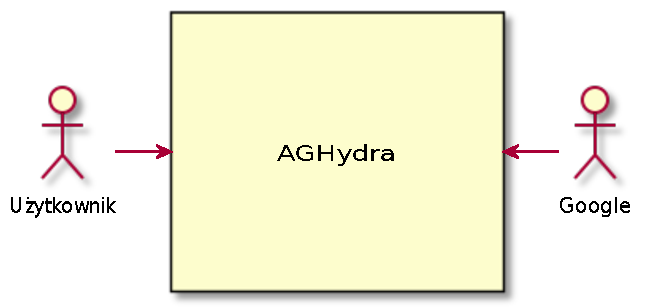
\includegraphics[width=\textwidth, keepaspectratio]{graphics/system_border.pdf}

\section{Lista możliwości}
\subsection{Obszar Wiki}
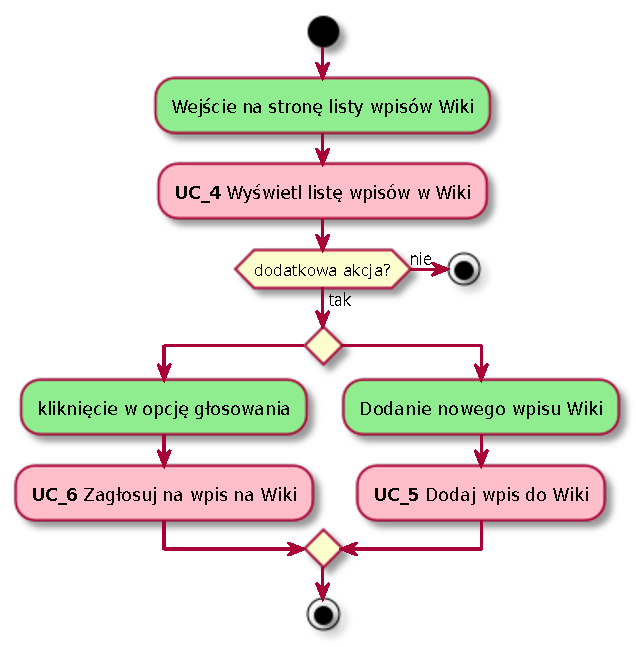
\includegraphics[width=\textwidth, keepaspectratio]{graphics/activity_diagram_wiki.pdf}

\subsection{Obszar Job i Referral}
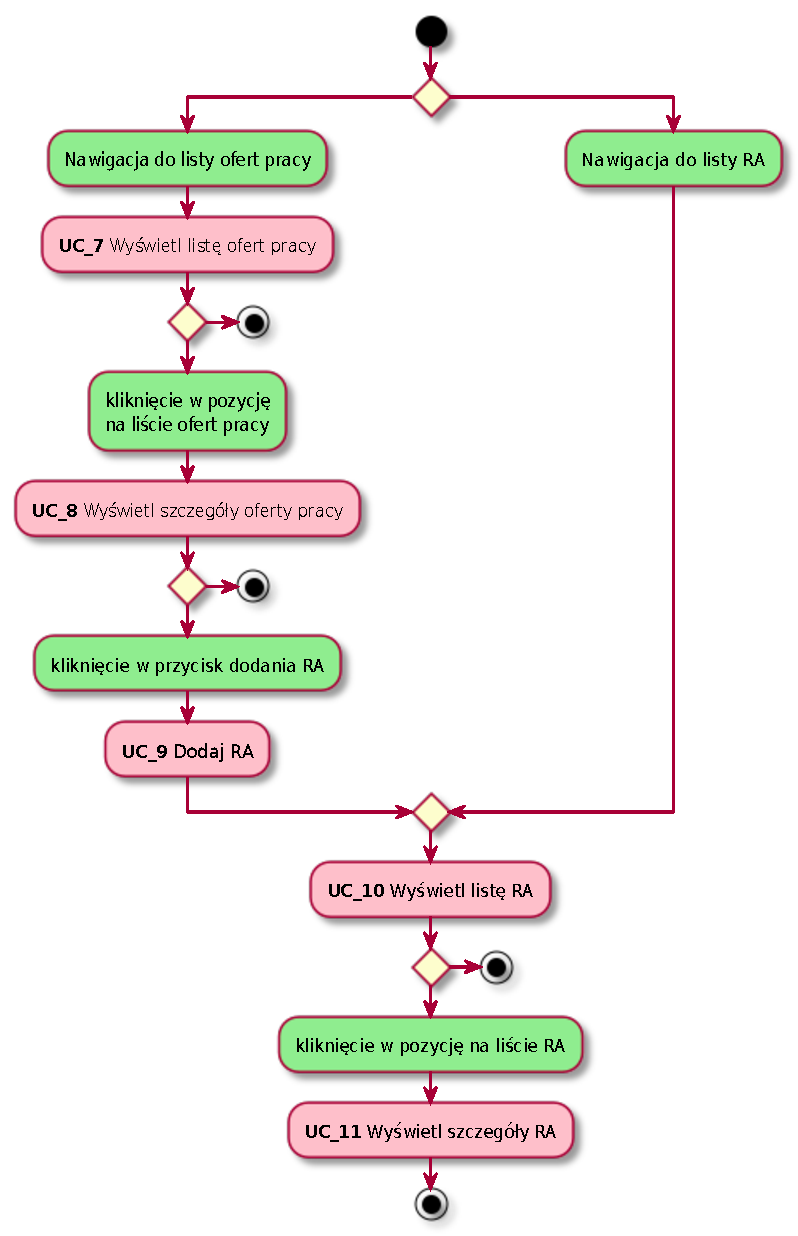
\includegraphics[width=\textwidth, keepaspectratio]{graphics/activity_diagram_job_referral.pdf}

\chapter{Analiza dziedziny}

\section{Diagram obiektów biznesowych}
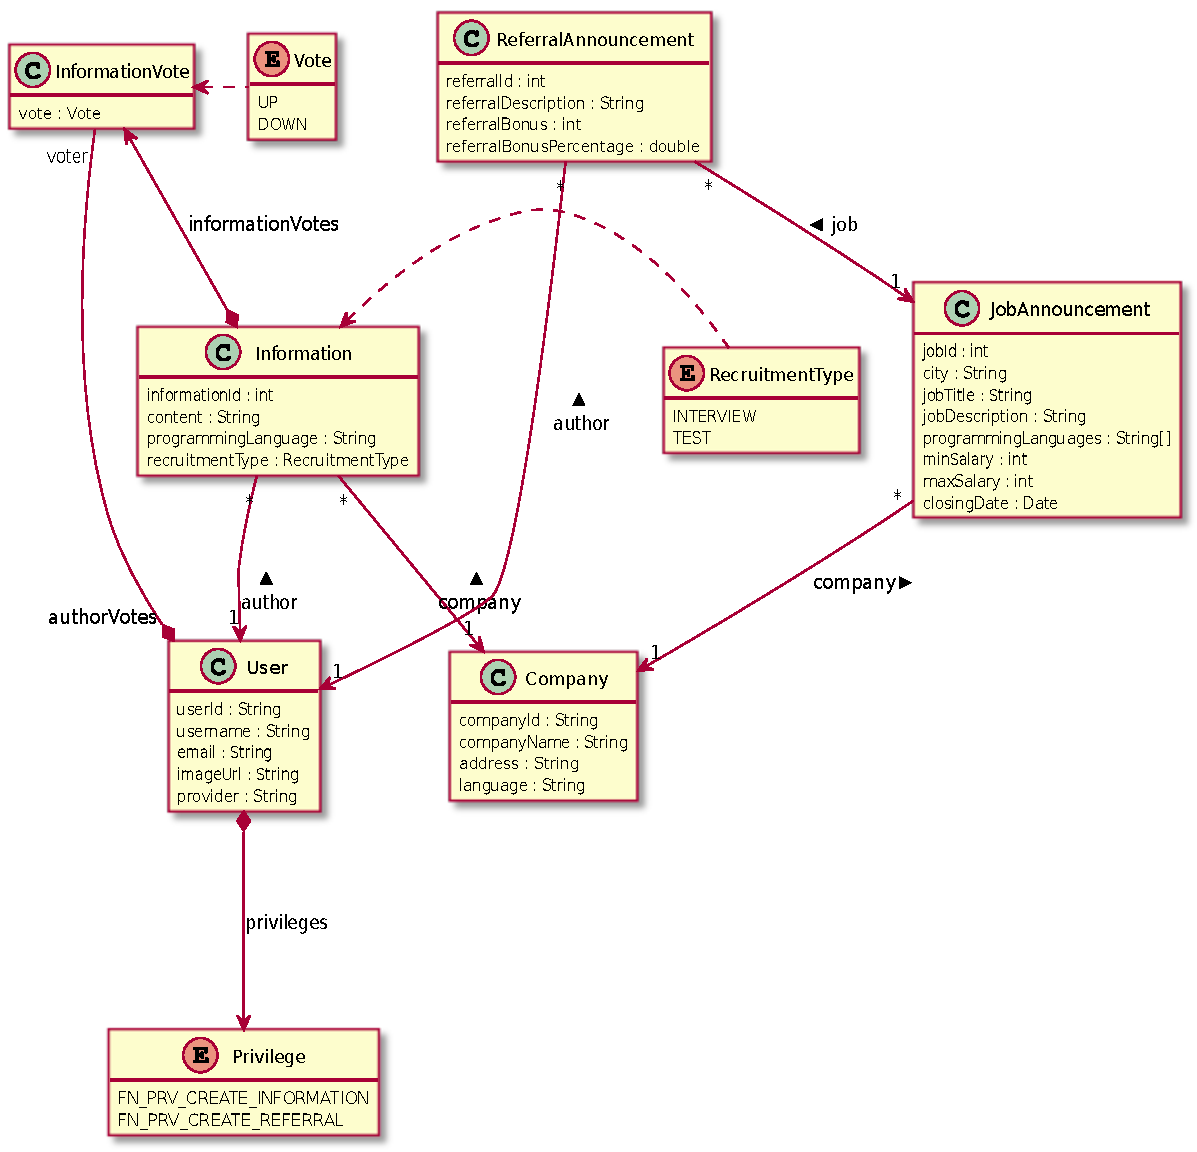
\includegraphics[width=\textwidth, keepaspectratio]{graphics/hydra_business_class_diagram.pdf}

\chapter{SRS - Specyfikacja wymagań}
\section{Diagram przypadków użycia - Wiki}
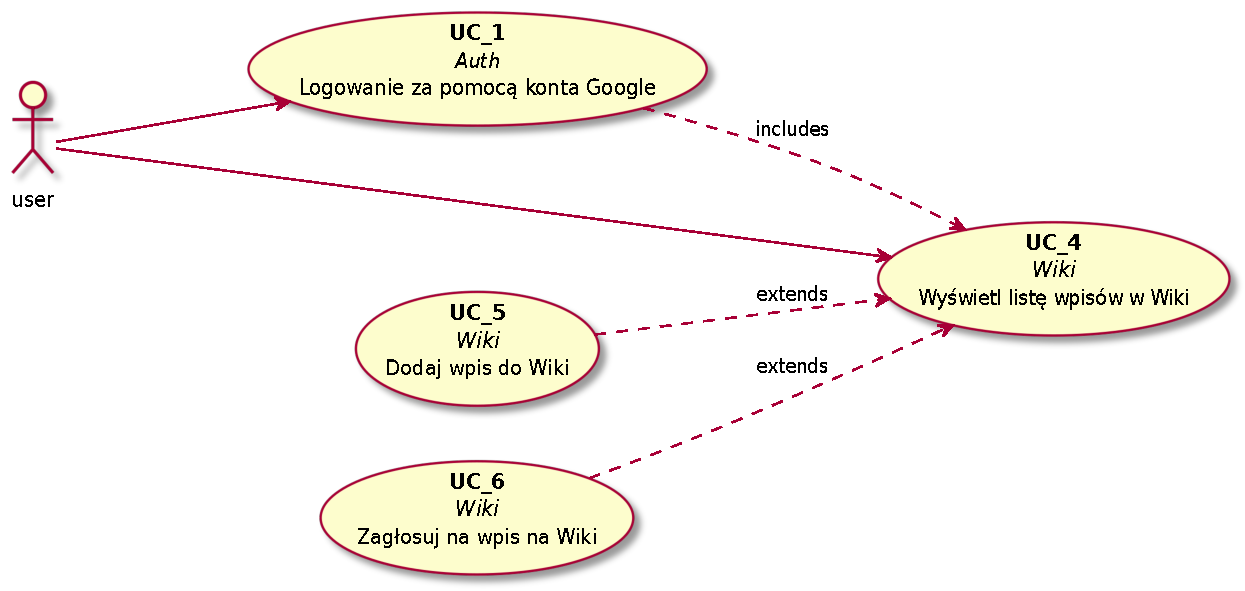
\includegraphics[width=\textwidth, keepaspectratio]{graphics/wiki_use_case_diagram.pdf}

\section{Diagram przypadków użycia - Job, Referral}
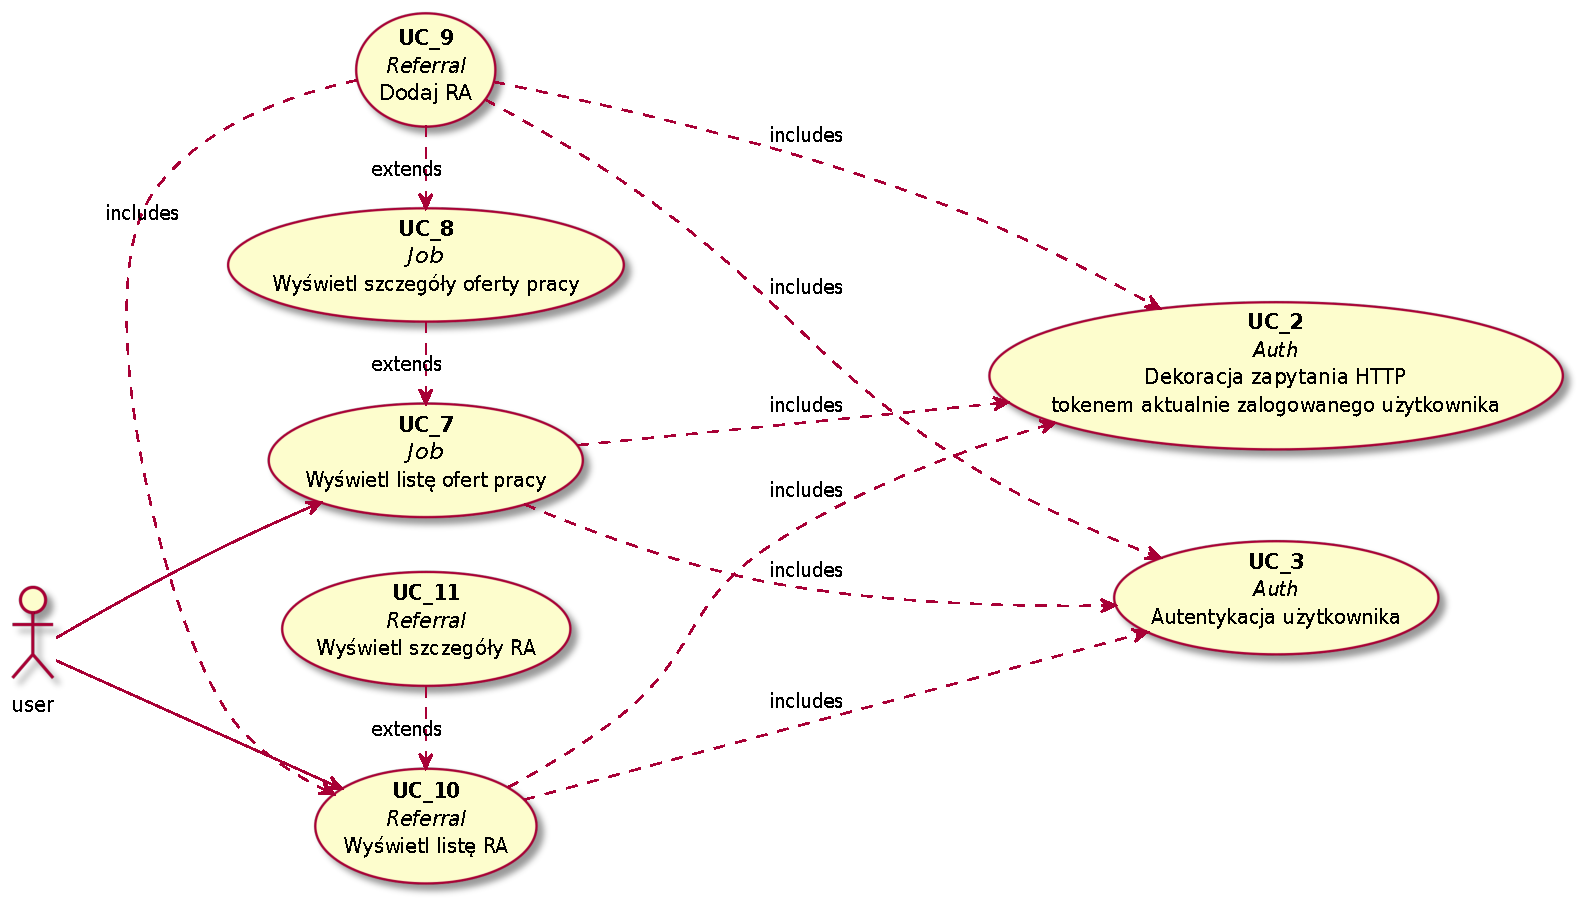
\includegraphics[width=\textwidth, keepaspectratio]{graphics/job_referral_use_case_diagram.pdf}

\section{Przypadki użycia powiązane z zabezpieczeniem dostępu}
\subsection{UC\_1 Logowanie za pomocą konta Google}

\begin{usecase}
	\addheading{Aktor}{Użytkownik, Google} 
	\addheading{Zakres}{System Hydra}
	\addheading{Poziom}{Systemowy}
	\addheading{Udziałowcy i ich cele}{Użytkownik chce zalogować się do Systemu}
	\addheading{Zdarzenie wyzwalające}{Użytkownik klika w przycisk logowania}
	\addheading{Warunki wstępne}{Użytkownik posiada konto w serwisie Google}
	\addheading{Warunki końcowe sukcesu}{Użytkownik zostaje poprawnie zalogowany}
	\addheading{Warunki końcowe porażki}{Użytkownik nie zostaje zalogowany, o czym informuje go komunikat}
	\addmulrow{Scenariusz główny (M)}{
		\item[] 1. Użytkownik klika przycisk logowania
		\item[] 2. System wywołuje serwis Google, w którym użytkownik dokonuje logowania na swoje konto Google
		\item[] 3. System weryfikuje zwrócony przez Google token po stronie serwera
		\item[] 4. Google zwraca dane użytkownika
		\item[] 5. System zapisuje dane o nowym użytkowniku
		\item[] 6. Przejście do UC\_4
	}
	\addmulrow{Scenariusz alternatywny}{
		\item[] 3.1 Google zwraca komunikat o błędzie
		\item[] 3.2 System wyświetla komunikat o niepowodzeniu weryfikacji
	}
	\addmulrow{Scenariusz alternatywny}{
		\item[] 4.1 Użytkownik istnieje już w systemie
		\item[] 4.2 Przejście do M.6
	}
\end{usecase}

\section{Przypadki użycia powiązane z Wiki}
\subsection{UC\_4 Wyświetl listę wpisów w Wiki}
\begin{usecase}
	\addheading{Aktor}{Użytkownik} 
	\addheading{Zakres}{System Hydra}
	\addheading{Poziom}{Systemowy}
	\addheading{Udziałowcy i ich cele}{Użytkownik chce wyświetlić wpisy wiki}
	\addheading{Zdarzenie wyzwalające}{Użytkownik zostaje przenawigowany do listy wpisów wiki}
	\addheading{Warunki wstępne}{Użytkownik jest poprawnie zalogowany}
	\addheading{Warunki końcowe sukcesu}{Użytkownikowi zostaje wyświetlona lista wpisów wiki}
	\addheading{Warunki końcowe porażki}{Użytkownik jest informowany o niepowodzeniu operacji}
	\addmulrow{Scenariusz główny (M)}{
		\item[] 1. Użytkownik nawiguje do strony z listą wpisów wiki
		\item[] 2. System wyświetla listę wpisów wiki
	}
\end{usecase}
\subsection{UC\_5 Dodaj wpis do Wiki}
\begin{usecase}
	\addheading{Aktor}{Użytkownik} 
	\addheading{Zakres}{System Hydra}
	\addheading{Poziom}{Systemowy}
	\addheading{Udziałowcy i ich cele}{Użytkownik chce dodać nowy wpis wiki}
	\addheading{Zdarzenie wyzwalające}{Użytkownik naciska przycisk dodania wpisu}
	\addheading{Warunki wstępne}{Użytkownik jest na stronie z załadowanymi wpisami wiki}
	\addheading{Warunki końcowe sukcesu}{Nowy wpis zostaje dodany}
	\addheading{Warunki końcowe porażki}{Nowy wpis nie zostaje dodany. Użytkownik jest informowany o niepowodzeniu operacji}
	\addmulrow{Scenariusz główny (M)}{
		\item[] 1. Użytkownik naciska przycisk dodania wpisu
		\item[] 2. System sprawdza czy użytkownik ma uprawnienie 'FN\_PRV\_CREATE\_INFORMATION'
		\item[] 3. System przenosi użytkownika do formularza nowego wpisu wiki
		\item[] 4. System ładuje dostępną listę firm do wyboru
		\item[] 5. Użytkownik wypełnia formularz i klika przycisk zatwierdzenia
		\item[] 6. System zapisuje nowy wpis
		\item[] 7. System przenosi użytkownika do poprzedniej strony
	}
	\addmulrow{Scenariusz alternatywny}{
		\item[] 2.1 Użytkownik nie posiada tego upranienia
		\item[] 2.2 System wyświetla komunikat z imformacją
	}
\end{usecase}

\subsection{UC\_6 Zagłosuj na wpis na Wiki}
\begin{usecase}
	\addheading{Aktor}{Użytkownik} 
	\addheading{Zakres}{System Hydra}
	\addheading{Poziom}{Systemowy}
	\addheading{Udziałowcy i ich cele}{Użytkownik chce zagłosować na wpis wiki}
	\addheading{Zdarzenie wyzwalające}{Użytkownik naciska opcję głosu}
	\addheading{Warunki wstępne}{Użytkownik jest na stronie z załadowanymi wpisami wiki}
	\addheading{Warunki końcowe sukcesu}{Głos użytkownika zostaje zapisany}
	\addheading{Warunki końcowe porażki}{Głos użytkownika nie zostaje zapisany}
	\addmulrow{Scenariusz główny (M)}{
		\item[] 1. Użytkownik wybiera jedną z trzech opcji głosowania
		\item[] 2. System zapisuje głos użytkownika
		\item[] 3. System aktualizuje widok listy wpisów wiki
	}
\end{usecase}

\section{Przypadki użycia powiązane z Job, Referral}
\subsection{UC\_7 Wyświetl listę ofert pracy}
\begin{usecase}
	\addheading{Aktor}{Użytkownik} 
	\addheading{Zakres}{System Hydra}
	\addheading{Poziom}{Systemowy}
	\addheading{Udziałowcy i ich cele}{Użytkownik chce wyświetlić oferty pracy}
	\addheading{Zdarzenie wyzwalające}{Użytkownik nawiguje do listy ofert pracy}
	\addheading{Warunki wstępne}{Użytkownik jest poprawnie zalogowany}
	\addheading{Warunki końcowe sukcesu}{Użytkownikowi zostaje wyświetlona lista ofert pracy}
	\addheading{Warunki końcowe porażki}{Użytkownik jest informowany o niepowodzeniu operacji}
	\addmulrow{Scenariusz główny (M)}{
		\item[] 1. Użytkownik nawiguje do strony z listą ofert pracy
		\item[] 2. System wyświetla listę aktualnych ofert pracy
	}
\end{usecase}

\subsection{UC\_8 Wyświetl szczegóły oferty pracy}
\begin{usecase}
	\addheading{Aktor}{Użytkownik} 
	\addheading{Zakres}{System Hydra}
	\addheading{Poziom}{Systemowy}
	\addheading{Udziałowcy i ich cele}{Użytkownik chce zobaczyć szczegóły oferty pracy}
	\addheading{Zdarzenie wyzwalające}{Użytkownik naciska na element listy ofert pracy}
	\addheading{Warunki wstępne}{Użytkownik jest na stronie z załadowanymi ofertami pracy}
	\addheading{Warunki końcowe sukcesu}{Użytkownik zostaje przeniesiony do strony szczegółów oferty pracy}
	\addmulrow{Scenariusz główny (M)}{
		\item[] 1. Użytkownik naciska na element listy ofert pracy
		\item[] 2. System przenosi użytkownika do strony szczegółów oferty pracy
	}
\end{usecase}

\subsection{UC\_9 Dodaj RA}
\begin{usecase}
	\addheading{Aktor}{Użytkownik} 
	\addheading{Zakres}{System Hydra}
	\addheading{Poziom}{Systemowy}
	\addheading{Udziałowcy i ich cele}{Użytkownik chce dodać nowe RA}
	\addheading{Zdarzenie wyzwalające}{Użytkownik naciska przycisk dodania RA}
	\addheading{Warunki wstępne}{Użytkownik jest na stronie z ze szczegółami oferty pracy}
	\addheading{Warunki końcowe sukcesu}{Nowe RA zostaje dodane}
	\addheading{Warunki końcowe porażki}{Nowe RA nie zostaje dodane. Użytkownik jest informowany o niepowodzeniu operacji}
	\addmulrow{Scenariusz główny (M)}{
		\item[] 1. Użytkownik naciska przycisk dodania RA
		\item[] 2. System sprawdza czy użytkownik ma uprawnienie 'FN\_PRV\_CREATE\_REFERRAL'
		\item[] 3. System przenosi użytkownika do formularza nowego RA
		\item[] 4. Użytkownik wypełnia formularz i klika przycisk zatwierdzenia
		\item[] 5. System zapisuje nowe RA
		\item[] 6. Przejście do UC\_10
	}
	\addmulrow{Scenariusz alternatywny}{
		\item[] 2.1 Użytkownik nie posiada tego upranienia
		\item[] 2.2 System wyświetla komunikat z imformacją
	}
	\addmulrow{Scenariusz alternatywny}{
		\item[] 4.1 Istnieje już aktywne RA przypisane do danej oferty pracy stworzone przez użytkownika
		\item[] 4.2 System wyświetla komunikat z imformacją
		\item[] 4.3 System przenosi użytkownika do poprzedniej strony
	}
\end{usecase}

\subsection{UC\_10 Wyświetl listę RA}
\begin{usecase}
	\addheading{Aktor}{Użytkownik} 
	\addheading{Zakres}{System Hydra}
	\addheading{Poziom}{Systemowy}
	\addheading{Udziałowcy i ich cele}{Użytkownik chce wyświetlić listę RA}
	\addheading{Zdarzenie wyzwalające}{Użytkownik zostaje przenawigowany do listy RA}
	\addheading{Warunki wstępne}{Użytkownik jest poprawnie zalogowany}
	\addheading{Warunki końcowe sukcesu}{Użytkownikowi zostaje wyświetlona lista RA}
	\addheading{Warunki końcowe porażki}{Użytkownik jest informowany o niepowodzeniu operacji}
	\addmulrow{Scenariusz główny (M)}{
		\item[] 1. Użytkownik nawiguje do strony z listą RA
		\item[] 2. System wyświetla listę aktualnych RA
	}
\end{usecase}

\subsection{UC\_11 Wyświetl szczegóły RA}
\begin{usecase}
	\addheading{Aktor}{Użytkownik} 
	\addheading{Zakres}{System Hydra}
	\addheading{Poziom}{Systemowy}
	\addheading{Udziałowcy i ich cele}{Użytkownik chce zobaczyć szczegóły RA}
	\addheading{Zdarzenie wyzwalające}{Użytkownik naciska na element listy RA}
	\addheading{Warunki wstępne}{Użytkownik jest na stronie z załadowanymi RA}
	\addheading{Warunki końcowe sukcesu}{Użytkownik zostaje przeniesiony do strony szczegółów RA}
	\addmulrow{Scenariusz główny (M)}{
		\item[] 1. Użytkownik naciska na element listy RA
		\item[] 2. System przenosi użytkownika do strony szczegółów RA
	}
\end{usecase}

\chapter{Architektura systemu}

\section{Diagram komponentów}
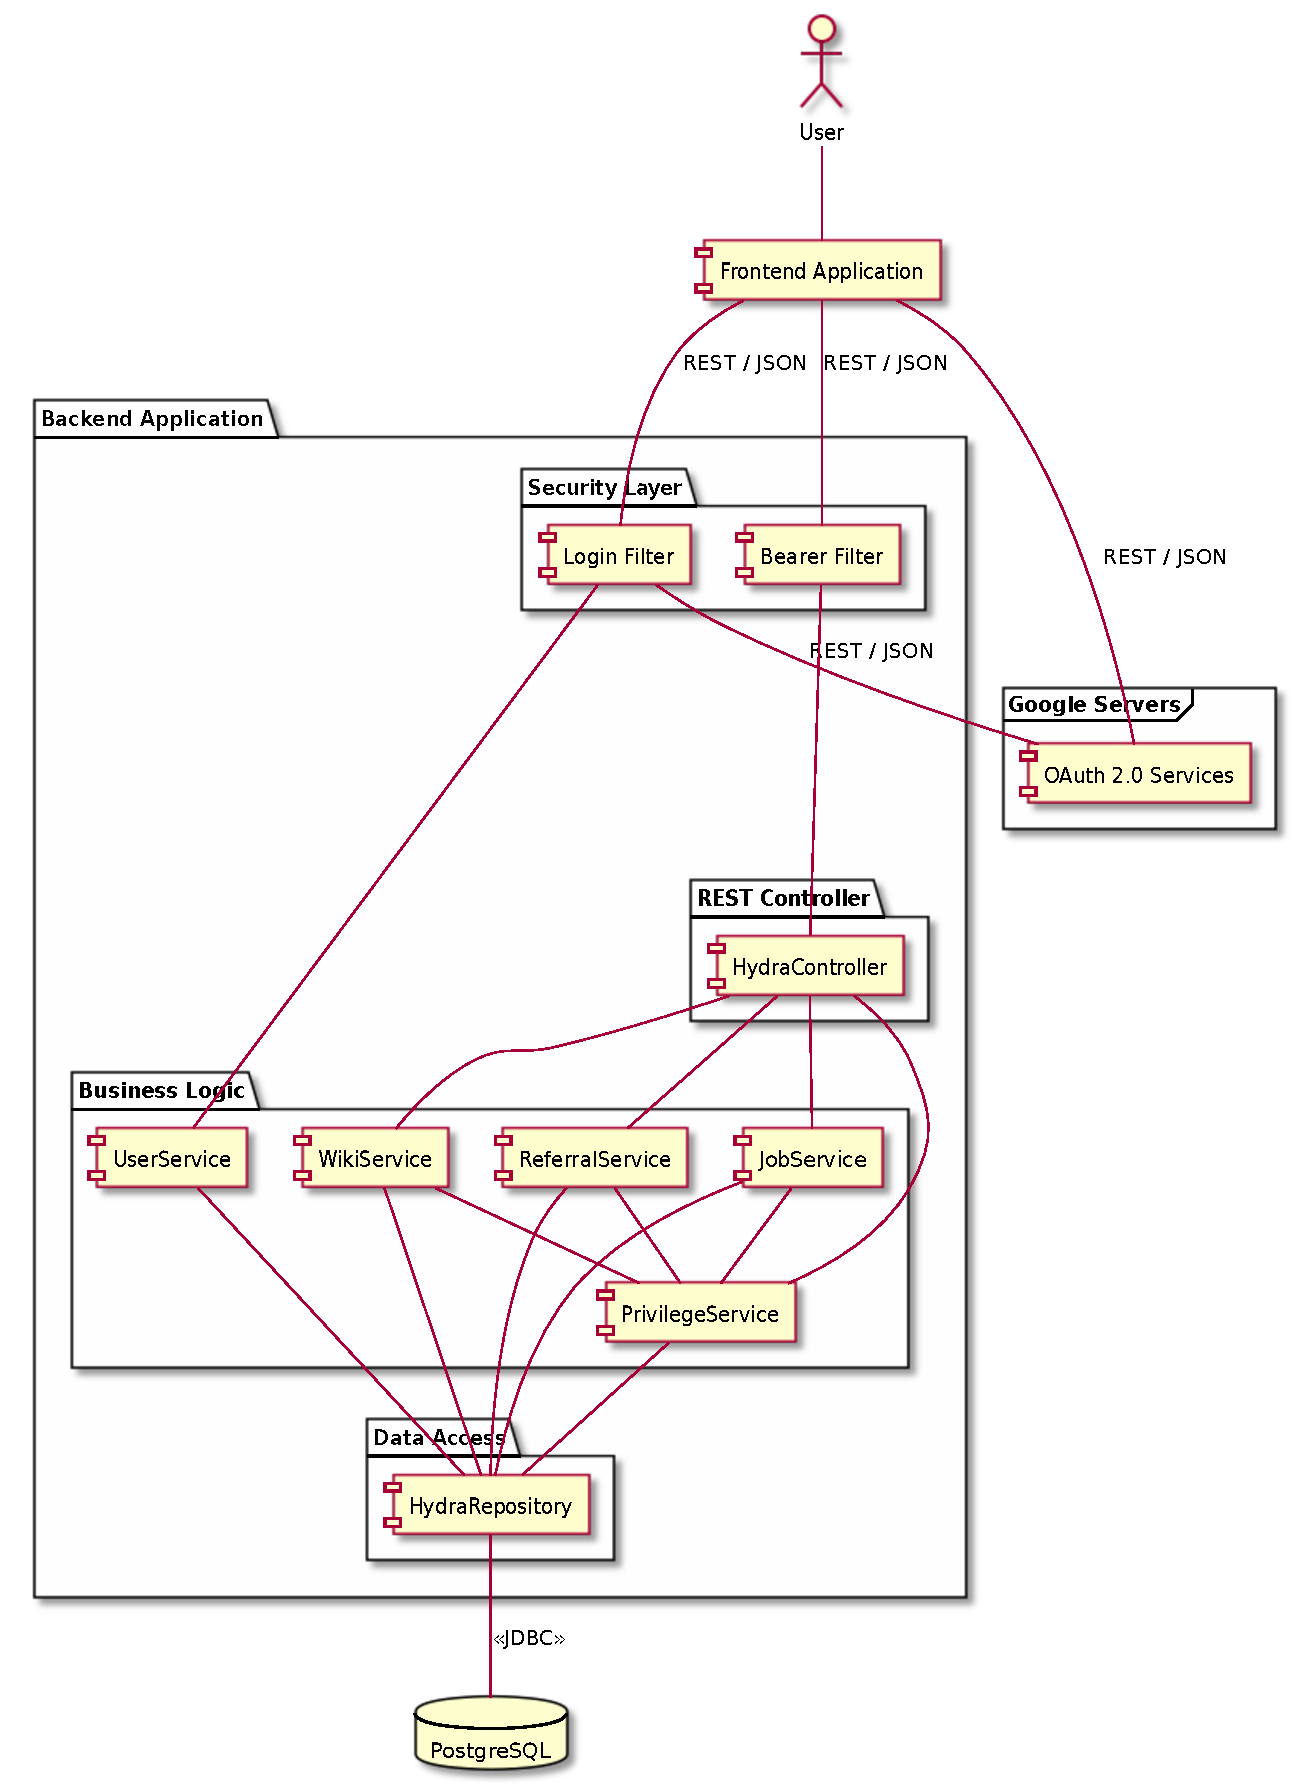
\includegraphics[width=\textwidth, keepaspectratio]{graphics/hydra_component_diagram.pdf}

\section{Opis warstw}
\subsection{Frontend Application}
Klient na platformy mobilne zrealizowany w języku \textbf{JavaScript} z wykorzystaniem frameworku \textbf{React Native}.
Pisany w ten sposób kod jest renderowany do natywnych implementacji Android \textit{(Java)} i iOS \textit{(Swift)}.

\subsection{Backend Application}
Serwer zrealizowany w technologii \textbf{Java} z wykorzystaniem biblioteki \textbf{Spring}

\subsubsection{Security Layer}
Warstwa odpowiada za zabezpieczenie dostępu do dalszych zasobów. 
Waliduje nadchodzące requesty na podstawie bearer tokena zawartego w ich nagłówkach.
Wychodząca odpowiedź serwera jest wzbogacana o odświeżony token i idektyfikator użytkownika.\\
Jedynym wyjątkiem w tym zabezpieczeniu jest próba logowania.

\subsubsection{REST Controller}
Komponenty te mapują zapytania do wywołań odpowiednich metod warstwy logiki biznesowej. 
Dodatkowo, nadchodzące requesty poddawane są walidacji pod kątem formatu zawartych danych.

\subsubsection{Business Logic}
Warstwa enkapsulująca logikę biznesową.

\subsubsection{Data Access}
Upraszcza innym komponentom integrację z informacjami przechowywanymi w bazie danych. 

\chapter{Projekt oprogramowania}

\subsection{Diagram klas}
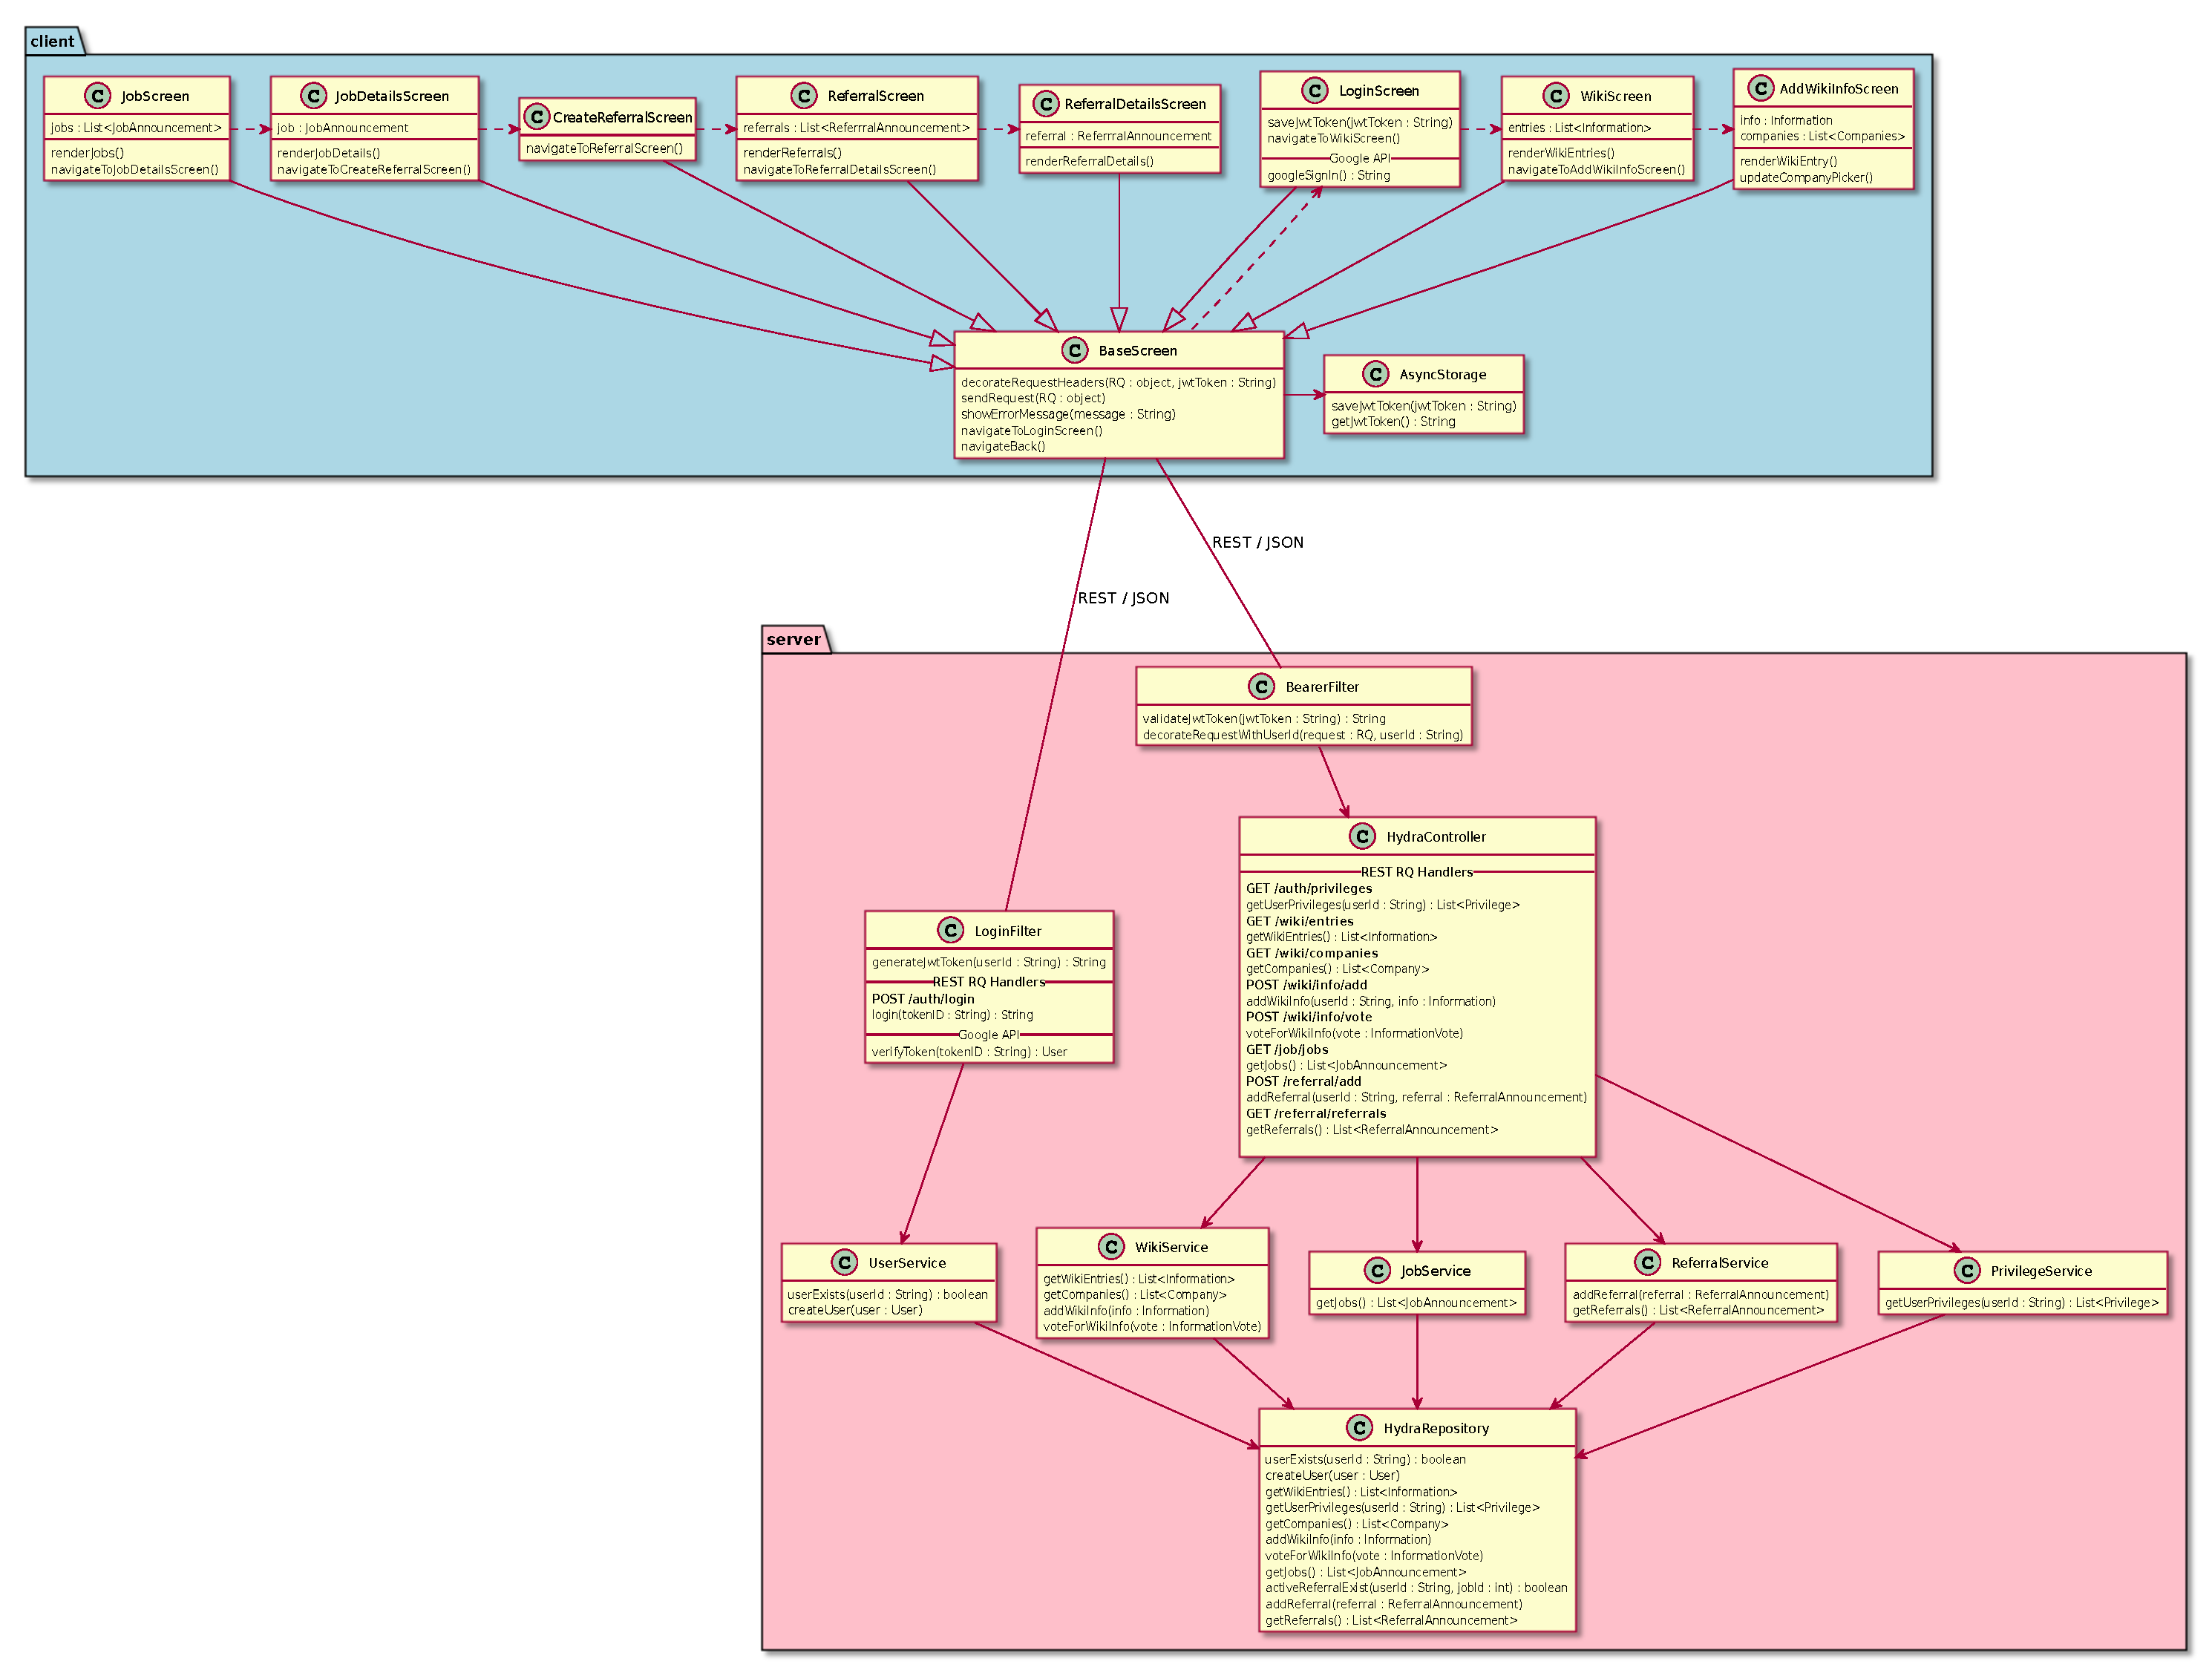
\includegraphics[width=\textwidth, keepaspectratio]{graphics/software_project_class_diagram.pdf}

\section{UC\_1 Logowanie za pomocą konta Google}
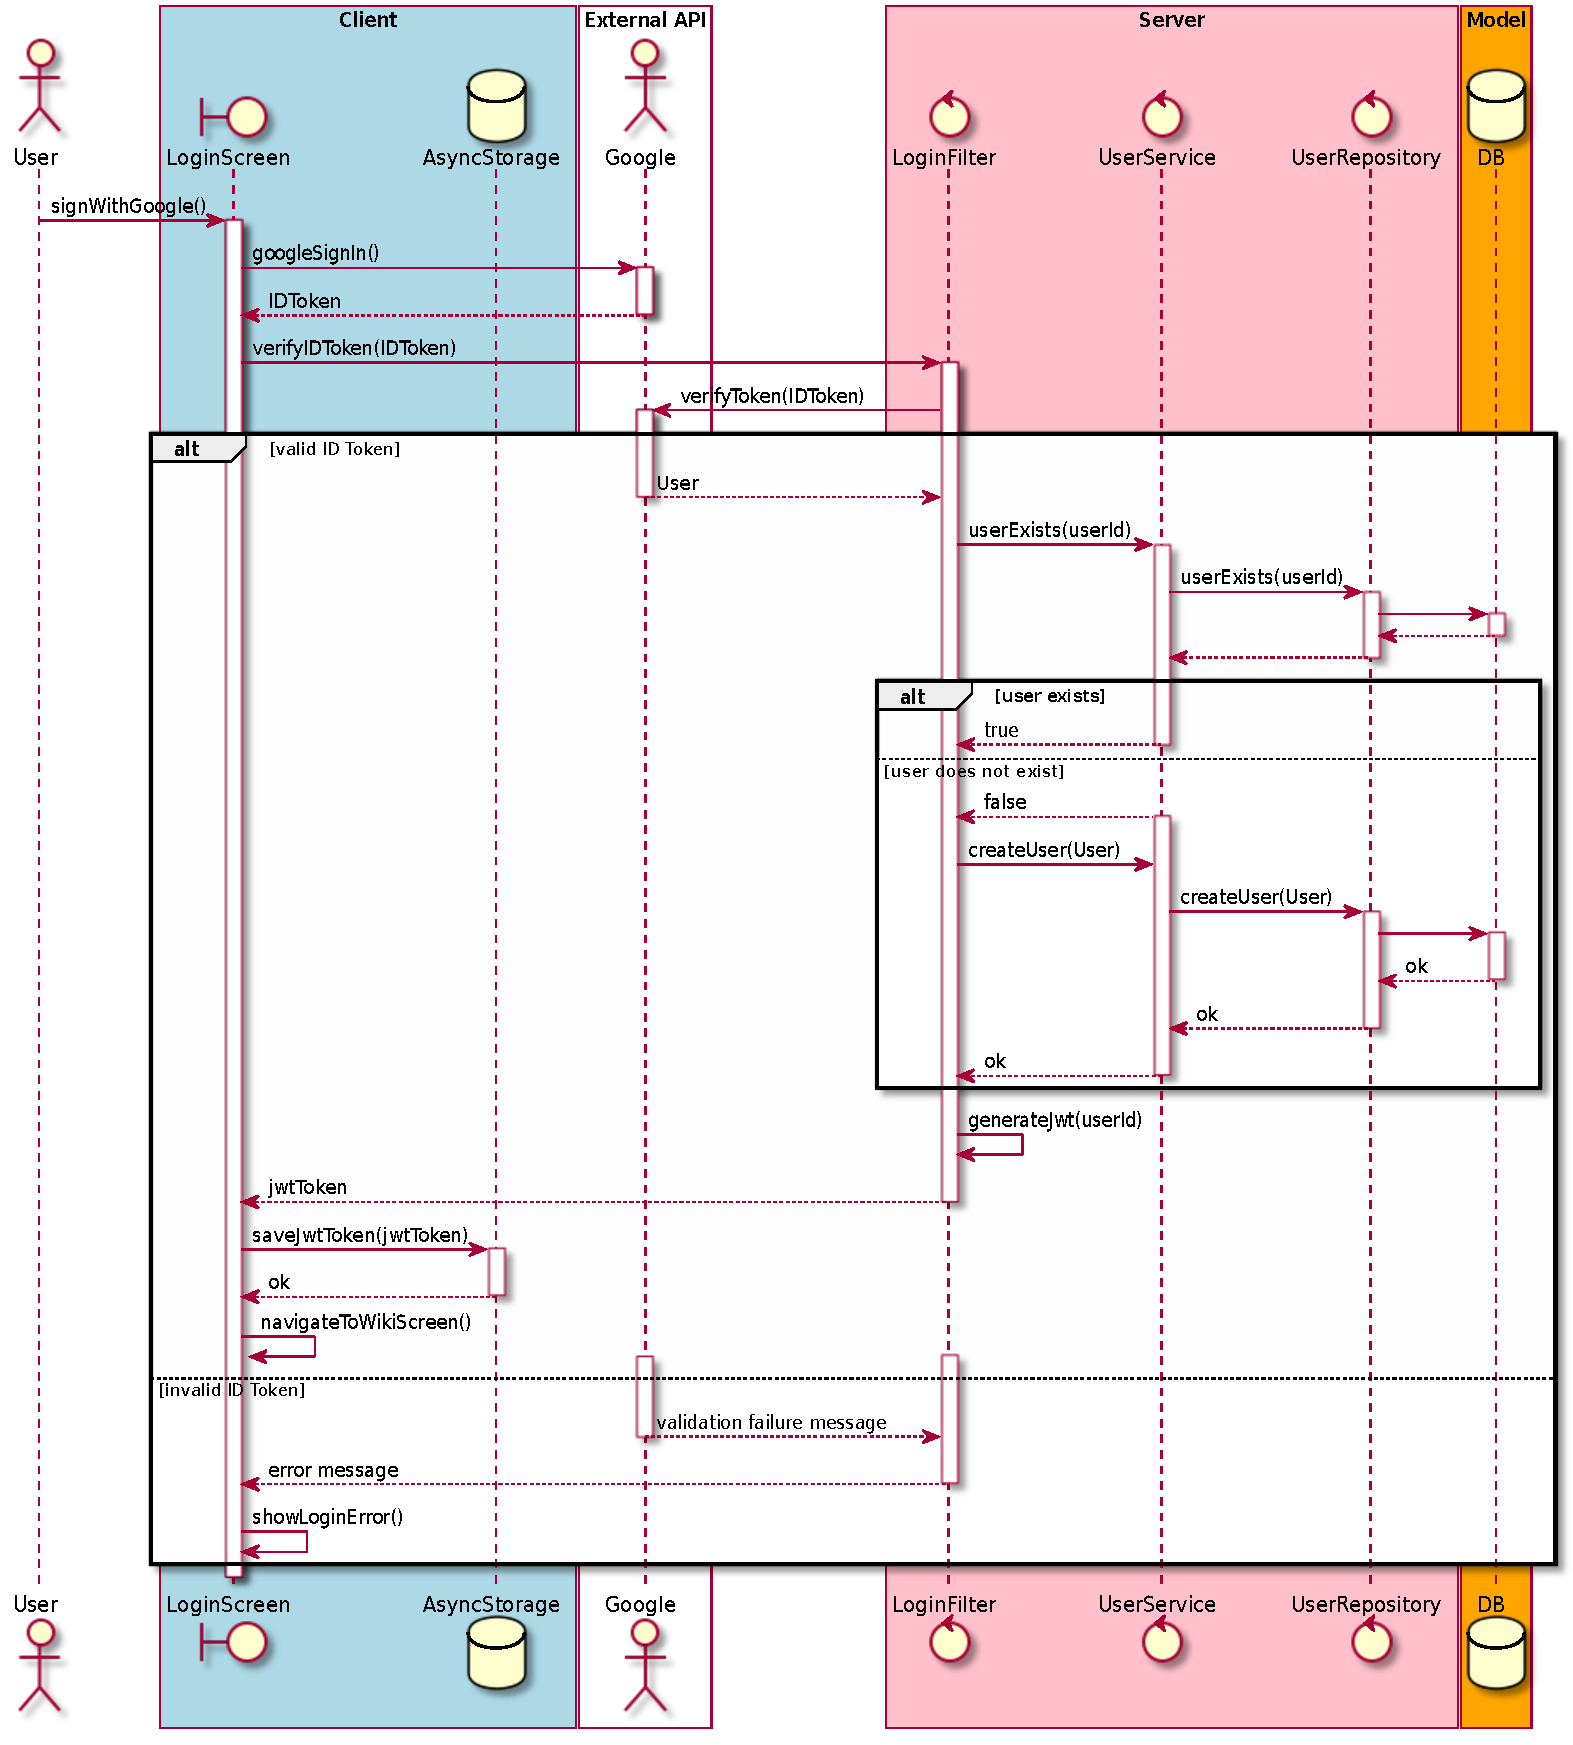
\includegraphics[width=\textwidth, keepaspectratio]{graphics/sequence_diagram_login.pdf}

\section{UC\_4 Wyświetl listę wpisów w Wiki}
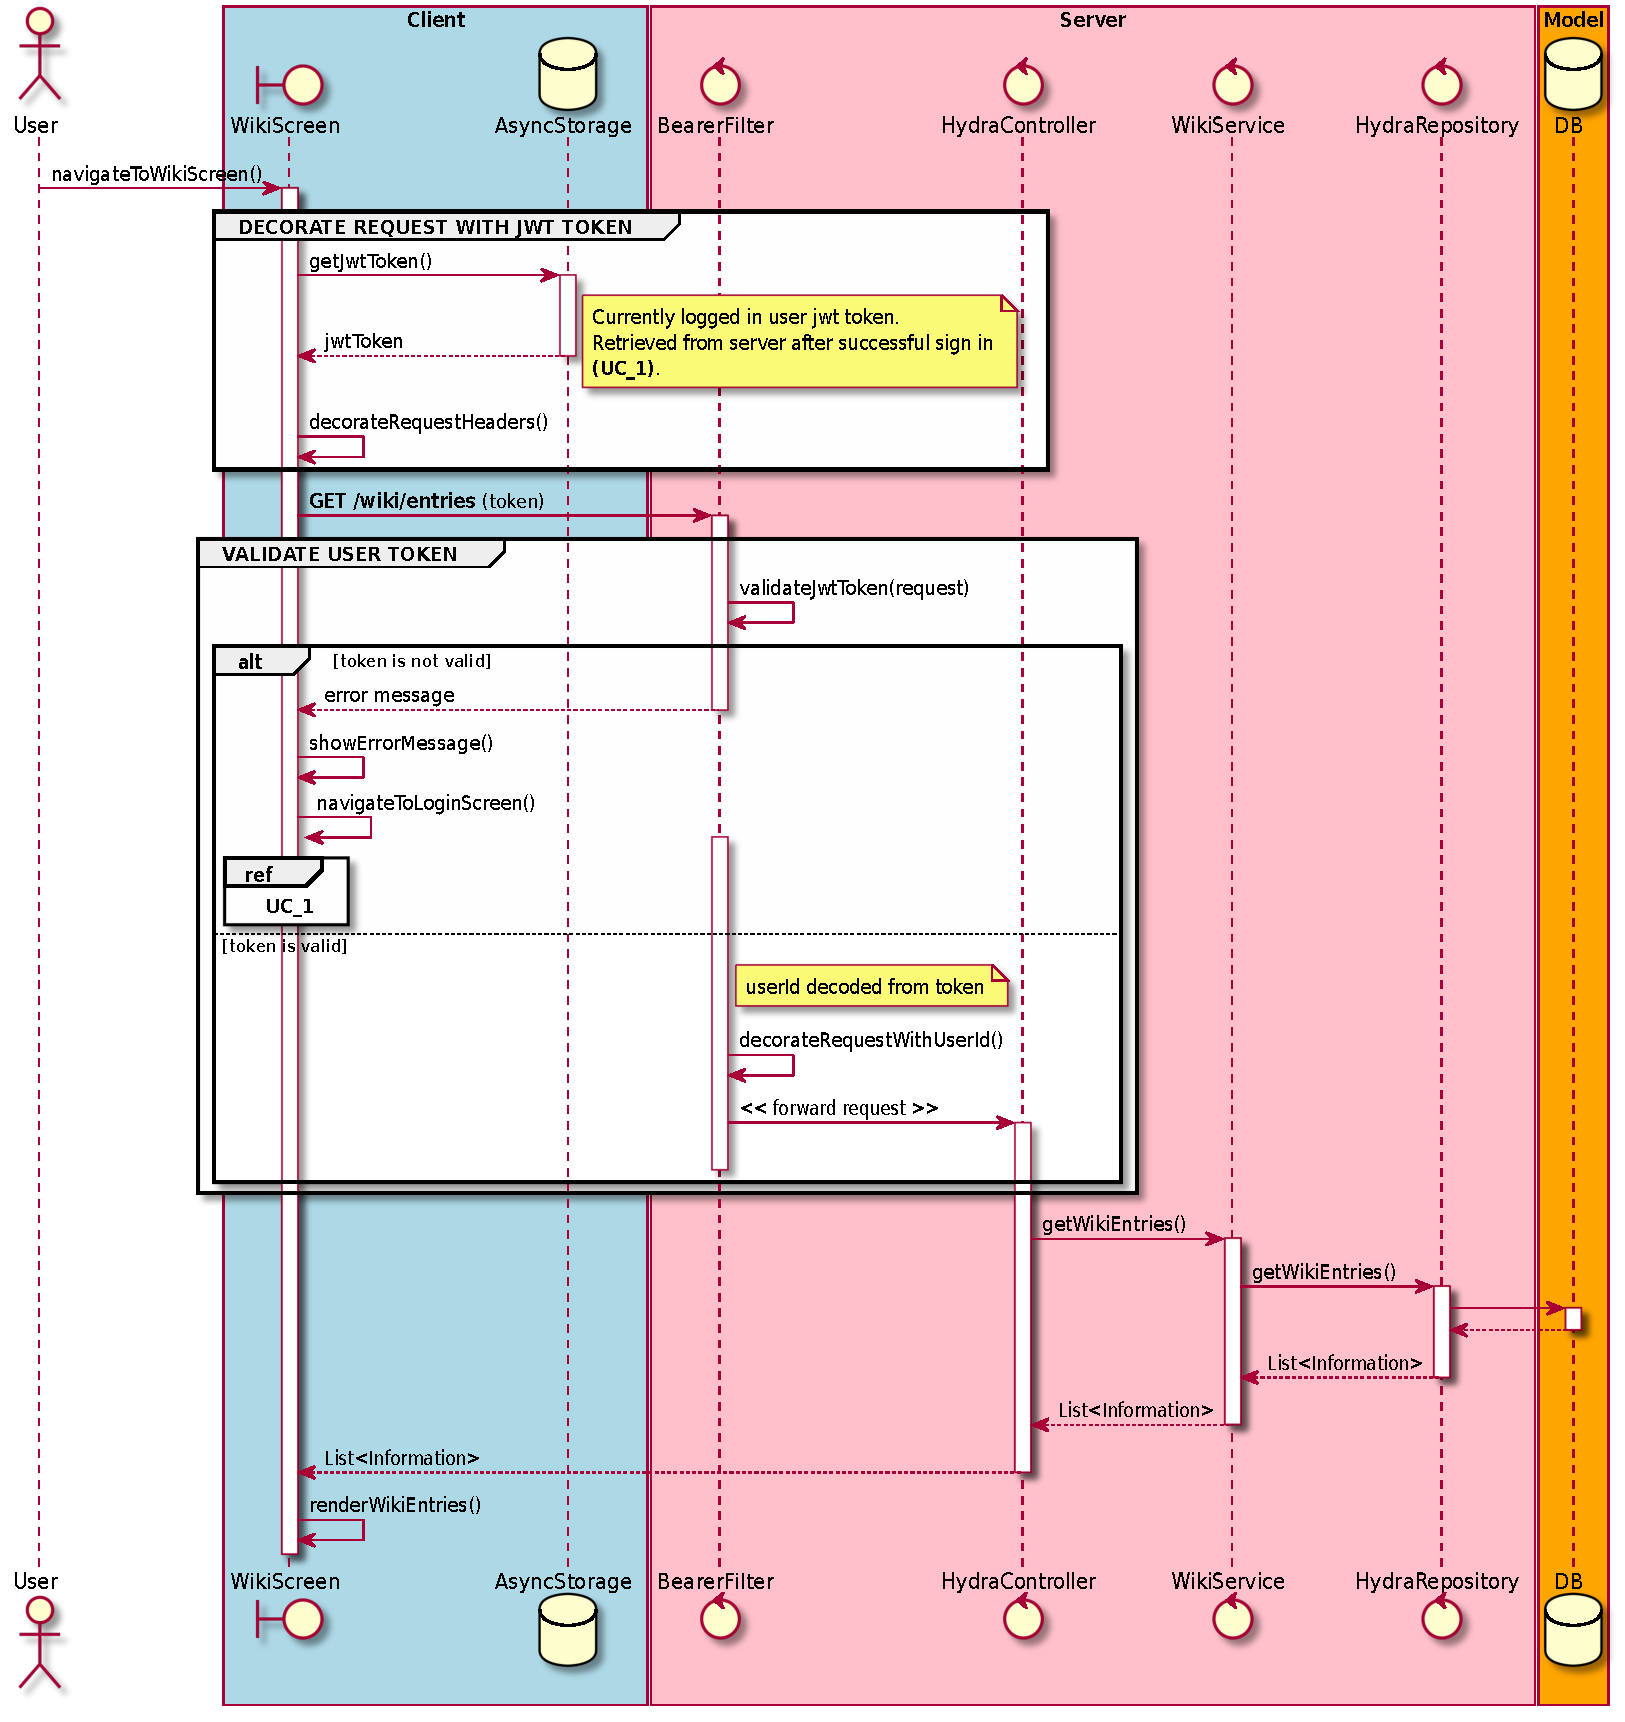
\includegraphics[width=\textwidth, keepaspectratio]{graphics/sequence_diagram_wiki_list.pdf}

\section{UC\_5 Dodaj wpis do Wiki}
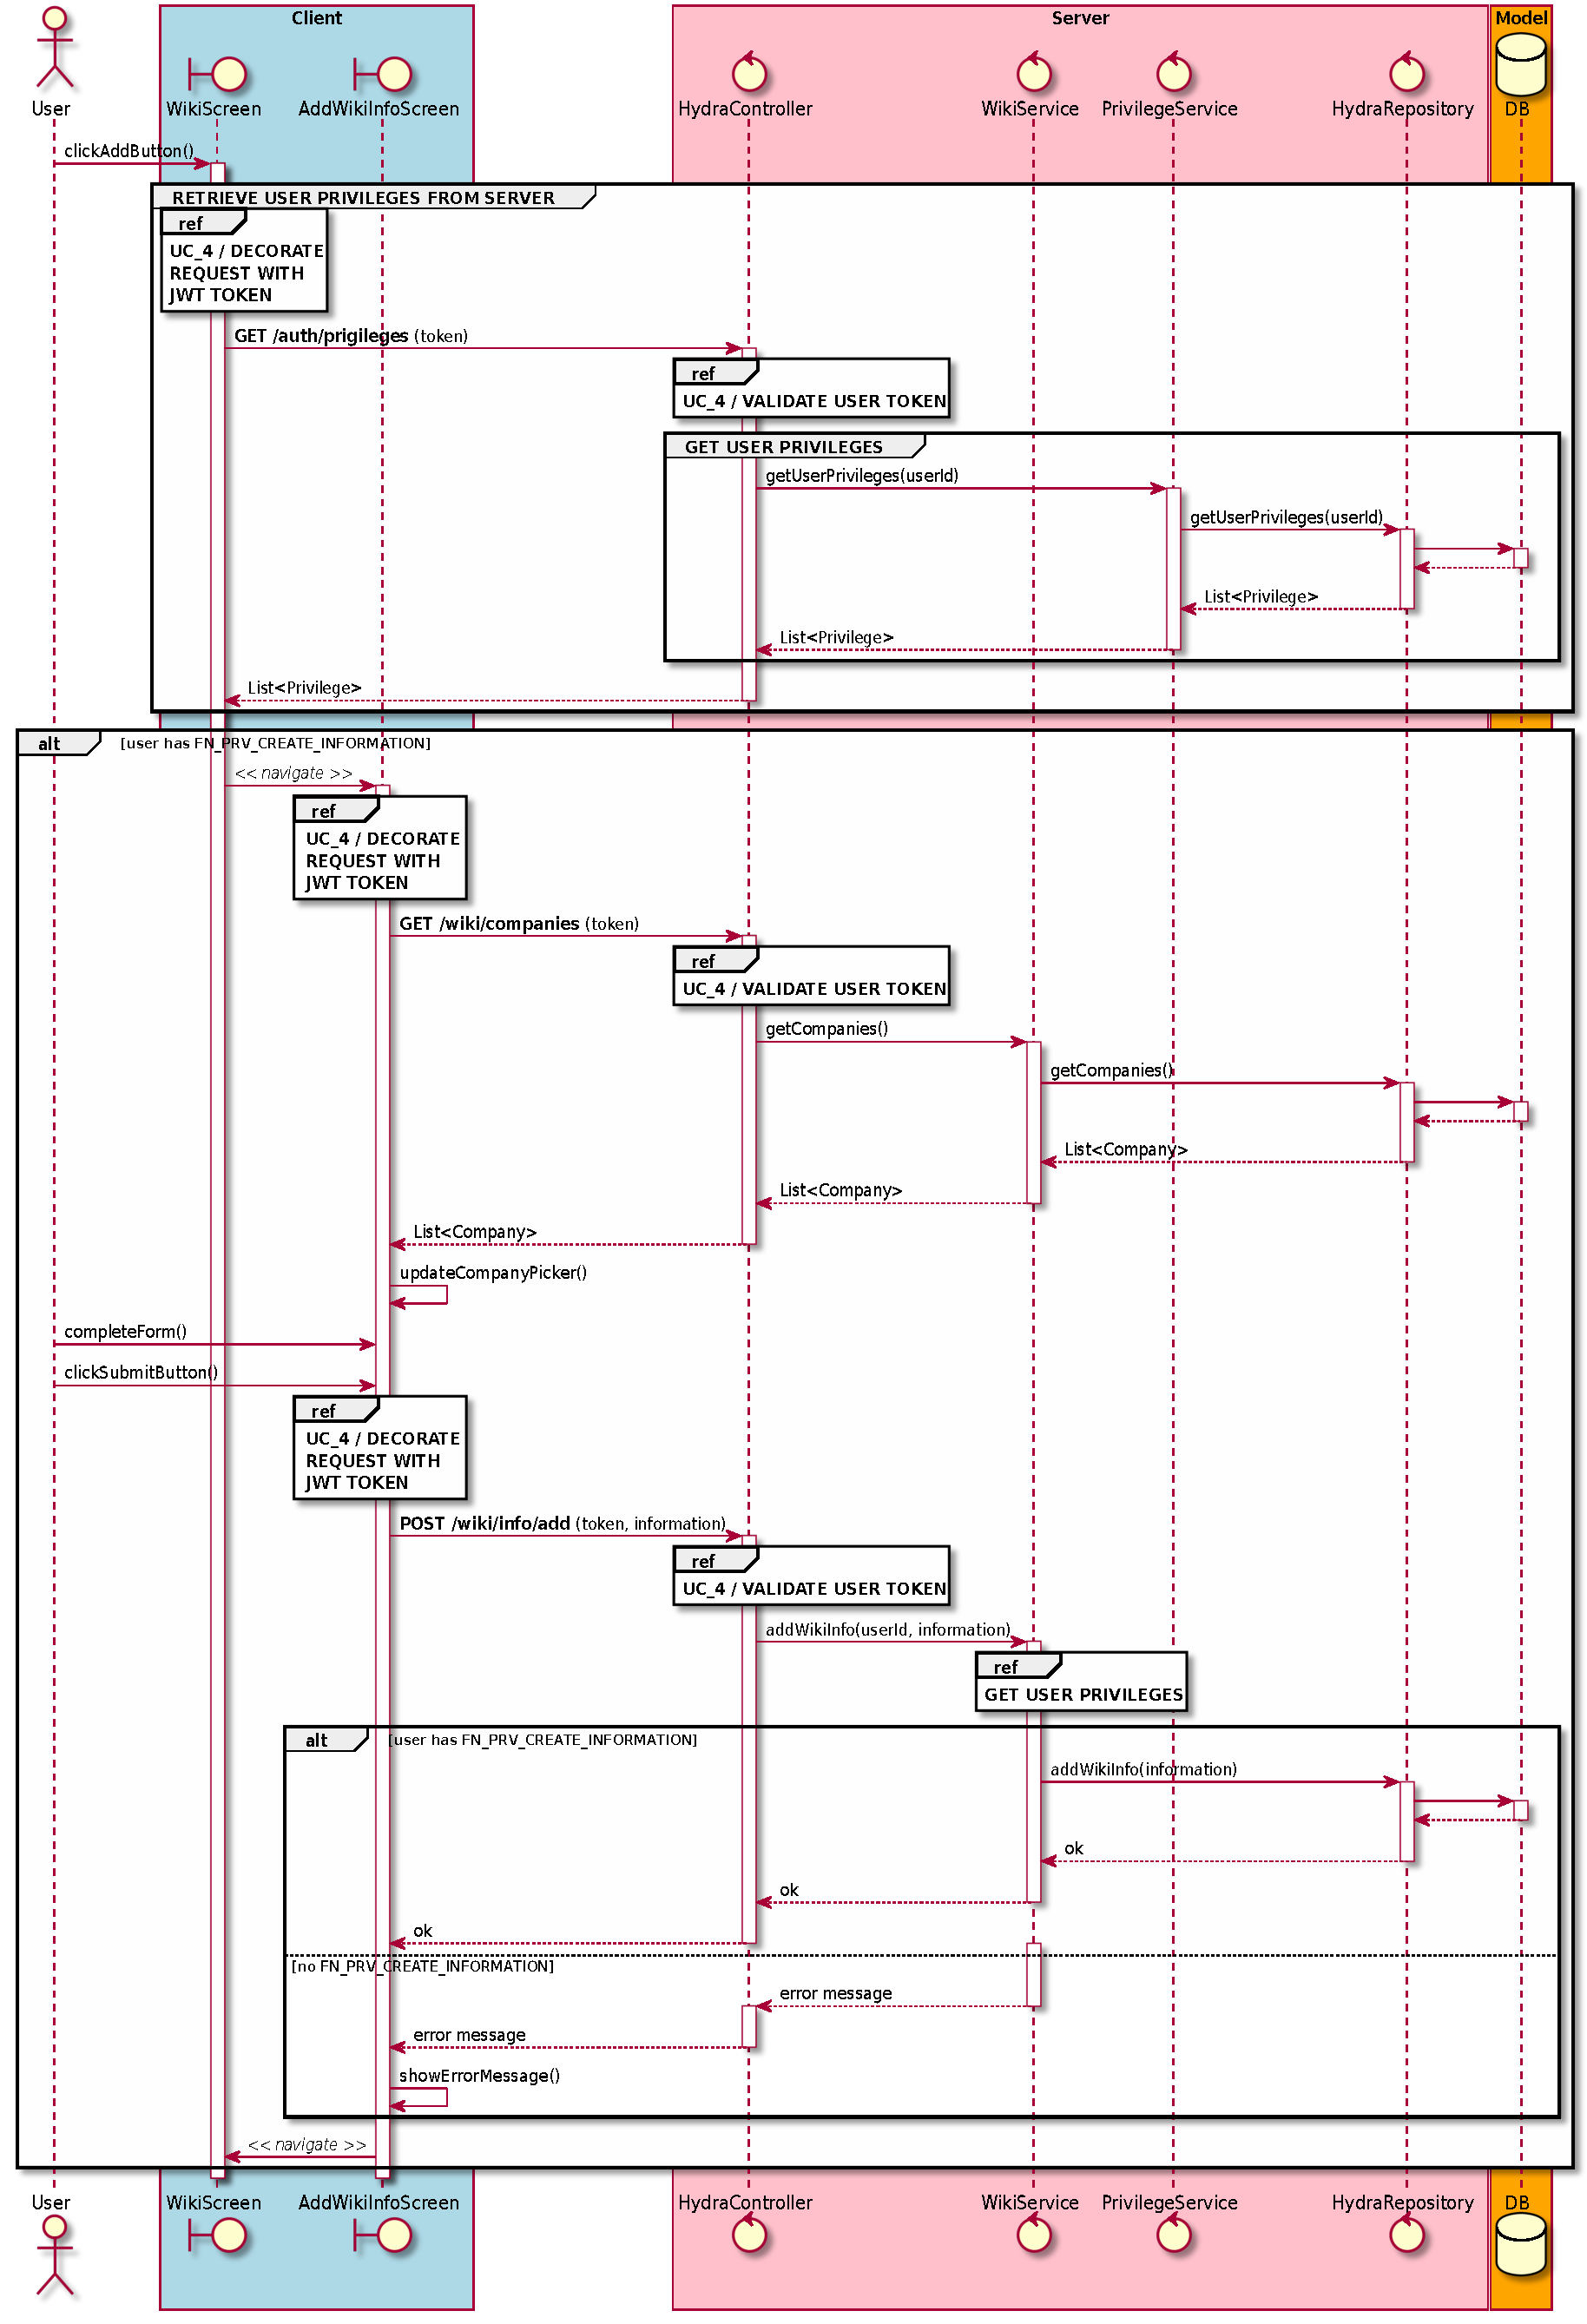
\includegraphics[width=\textwidth, keepaspectratio]{graphics/sequence_diagram_wiki_add.pdf}

\section{UC\_6 Zagłosuj na wpis na Wiki}
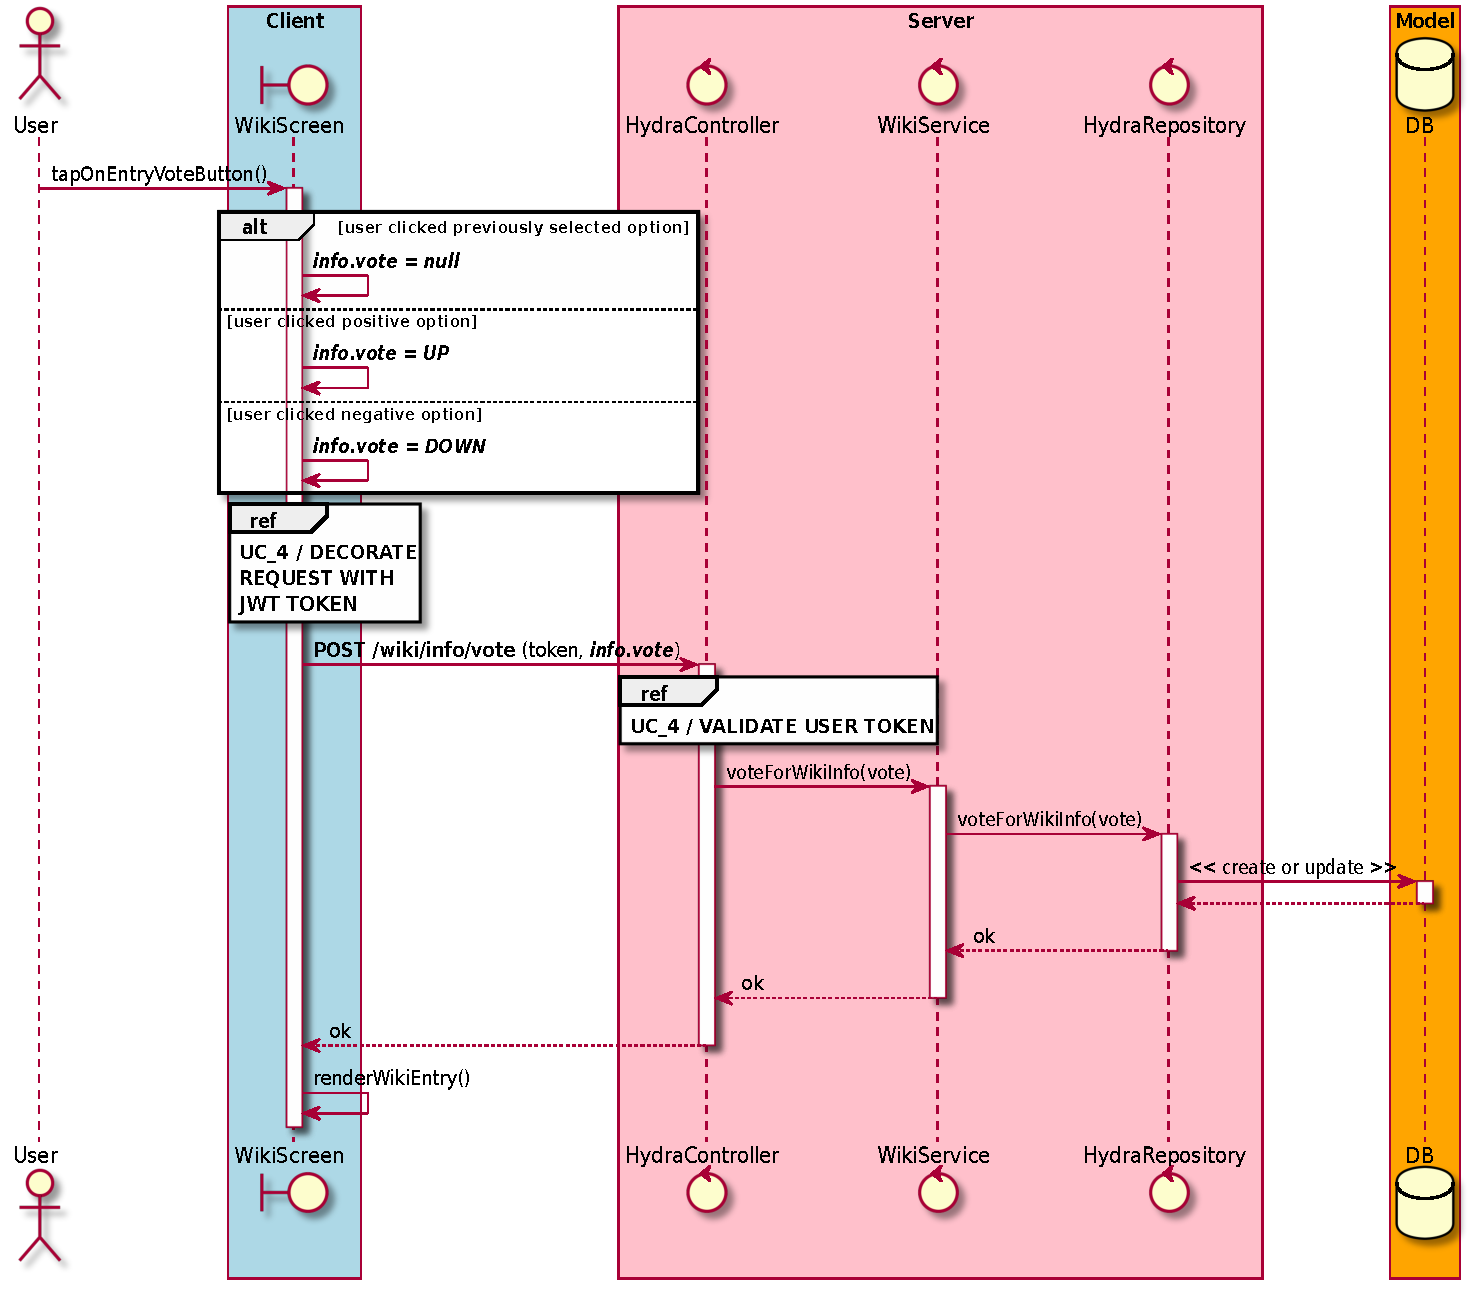
\includegraphics[width=\textwidth, keepaspectratio]{graphics/sequence_diagram_wiki_vote.pdf}

\section{UC\_7 Wyświetl listę ofert pracy}
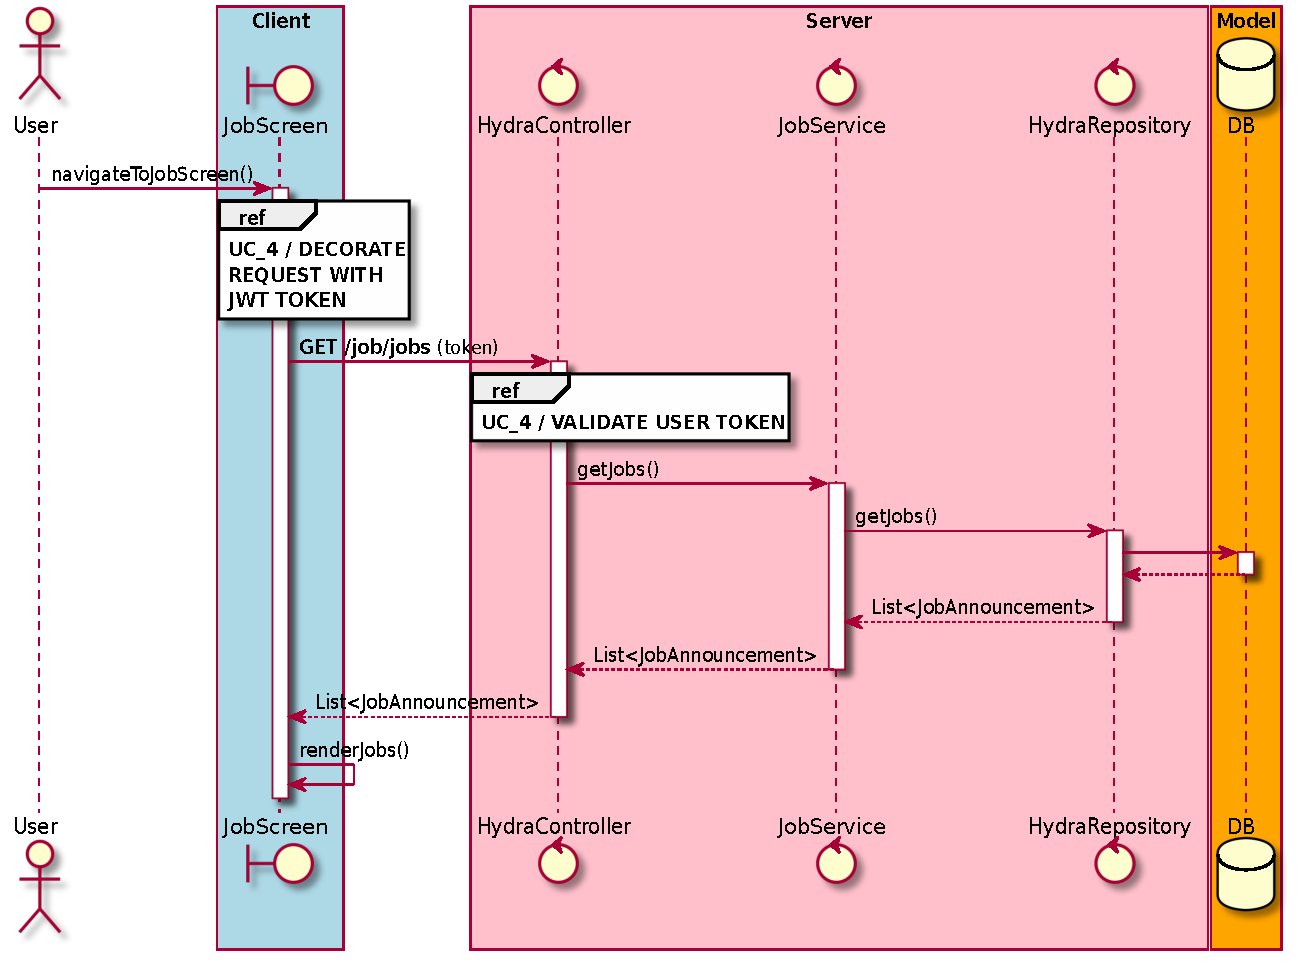
\includegraphics[width=\textwidth, keepaspectratio]{graphics/sequence_diagram_job_list.pdf}

\section{UC\_8 Wyświetl szczegóły oferty pracy}
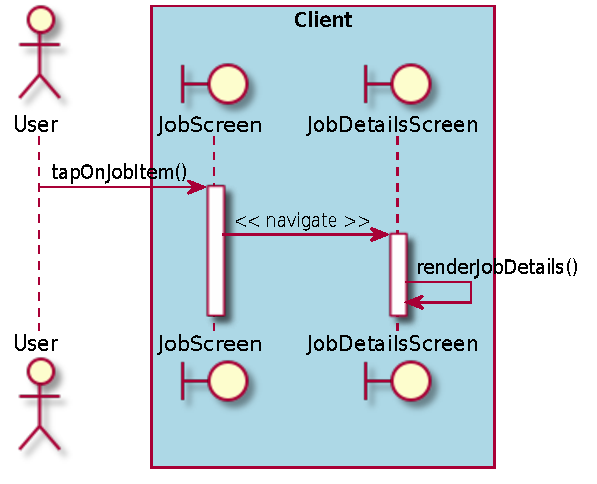
\includegraphics[width=\textwidth, keepaspectratio]{graphics/sequence_diagram_job_details.pdf}

\section{UC\_9 Dodaj RA}
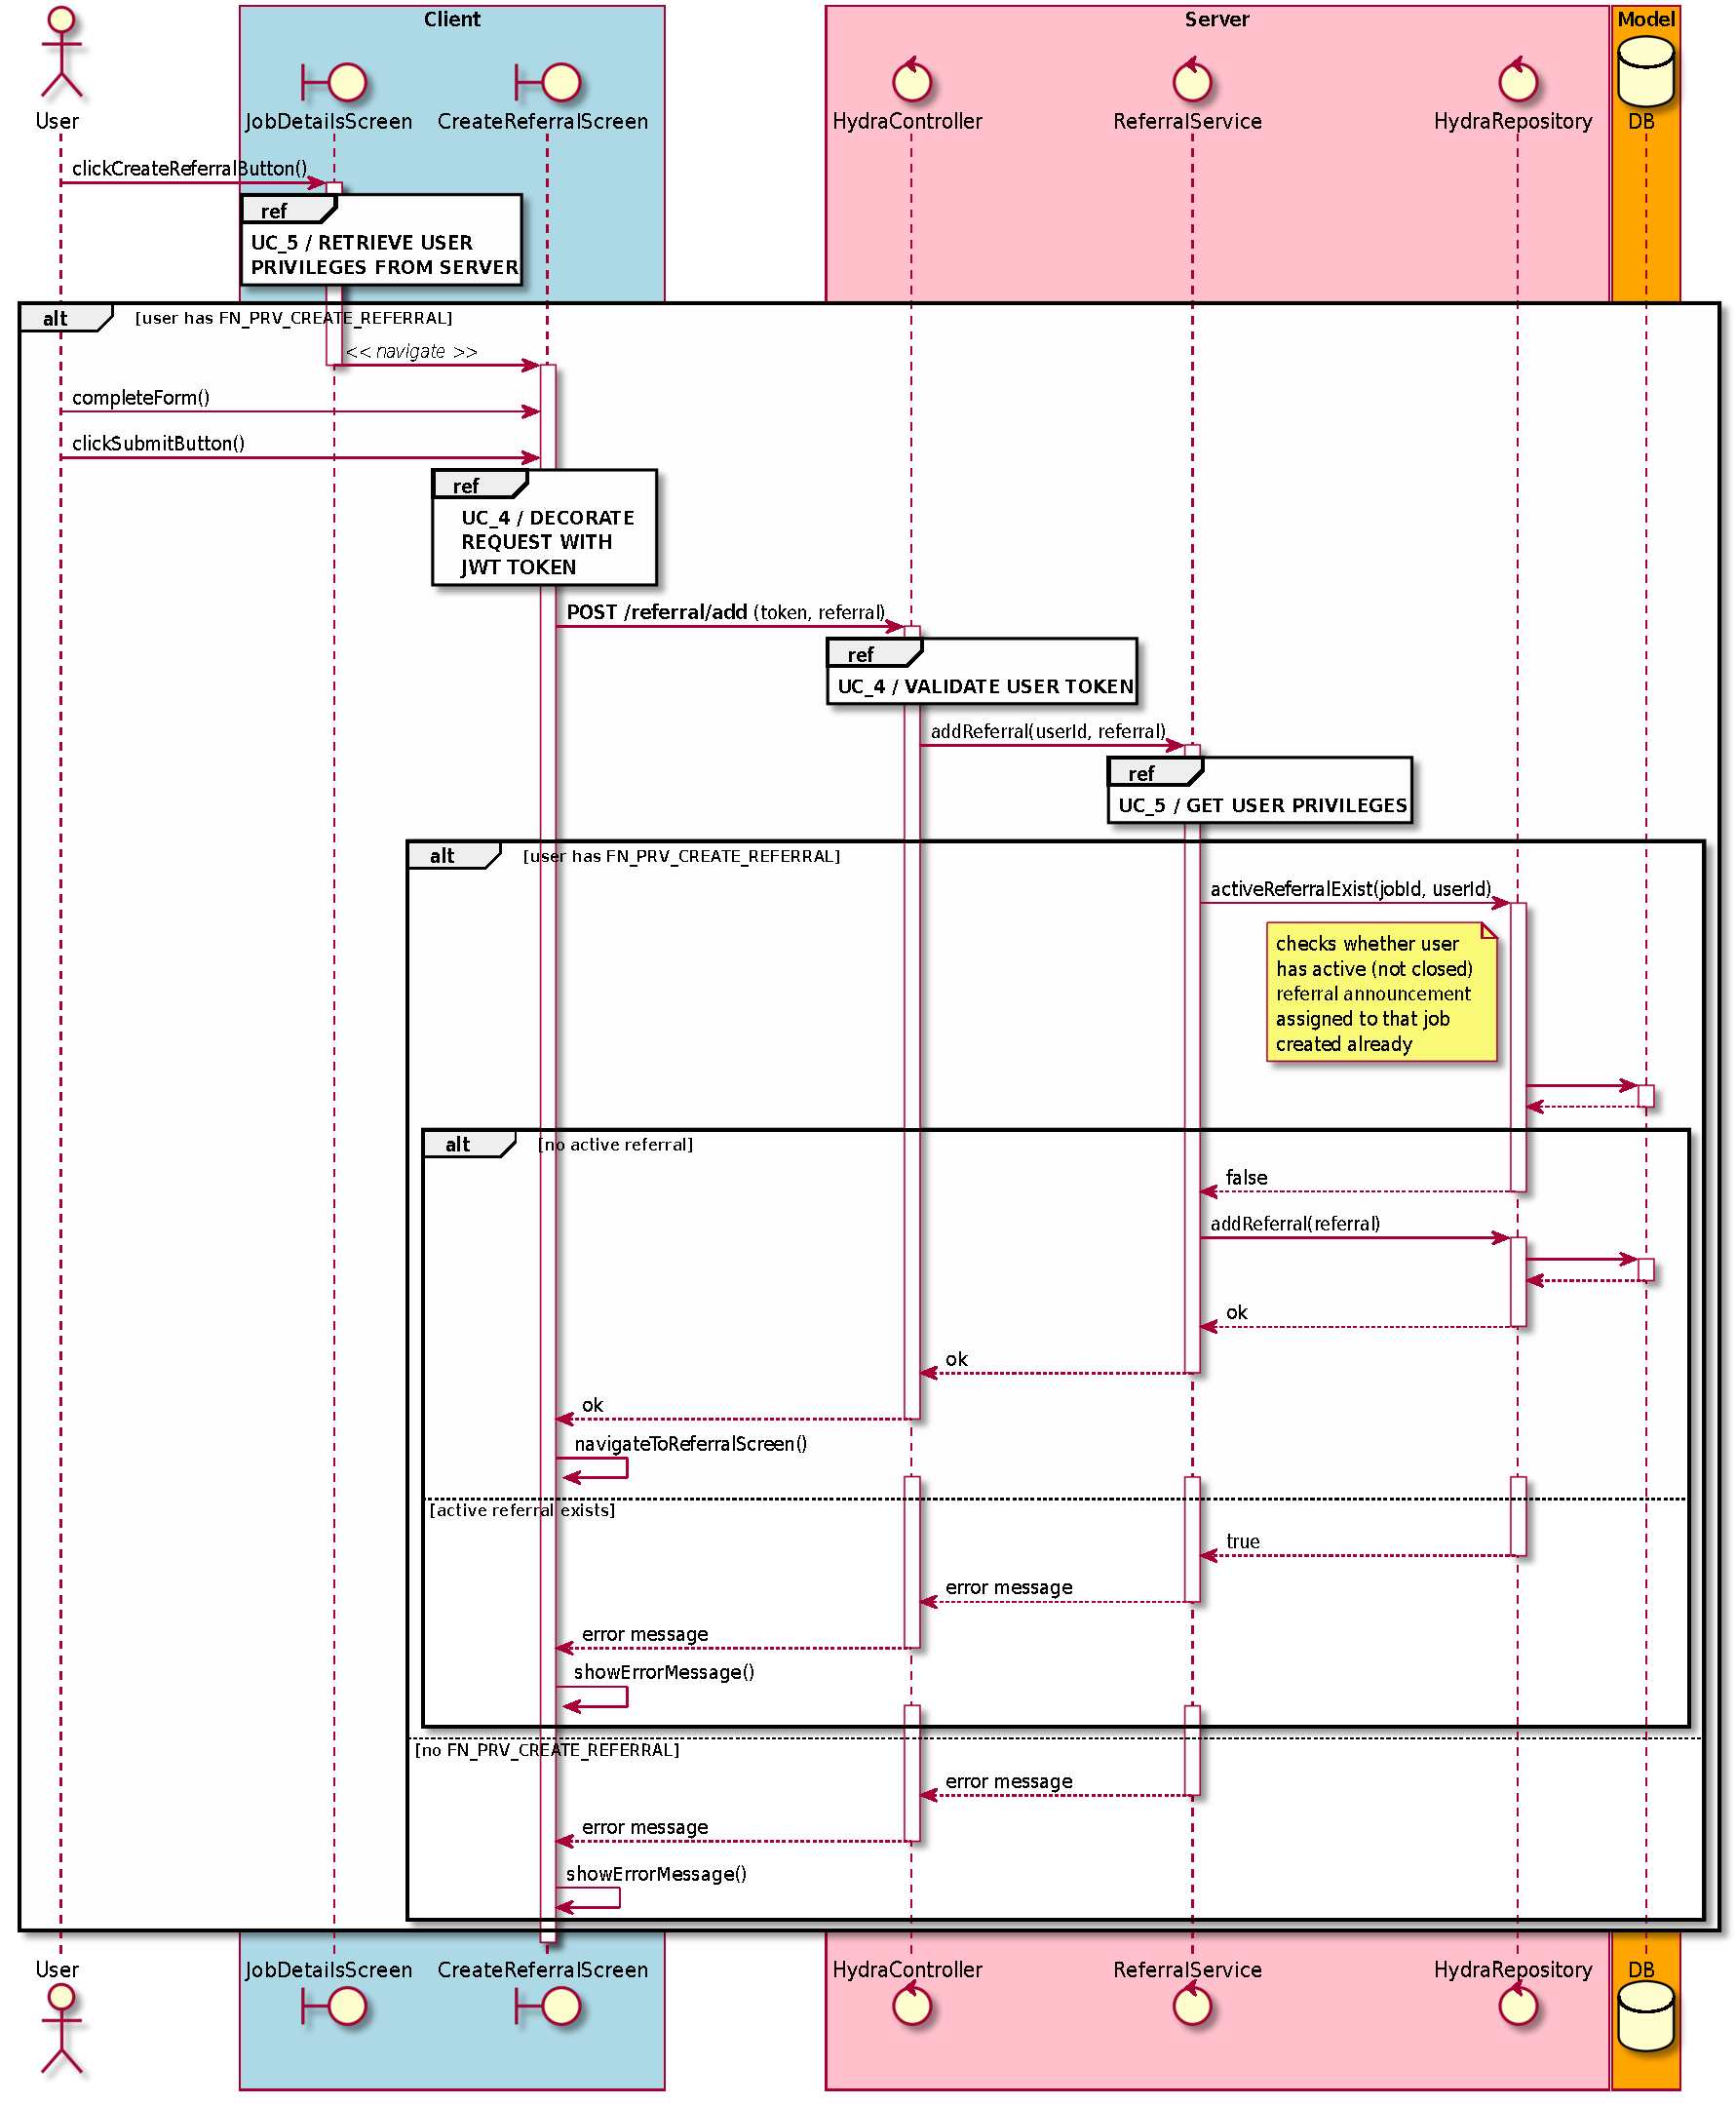
\includegraphics[width=\textwidth, keepaspectratio]{graphics/sequence_diagram_referral_add.pdf}

\section{UC\_10 Wyświetl listę RA}
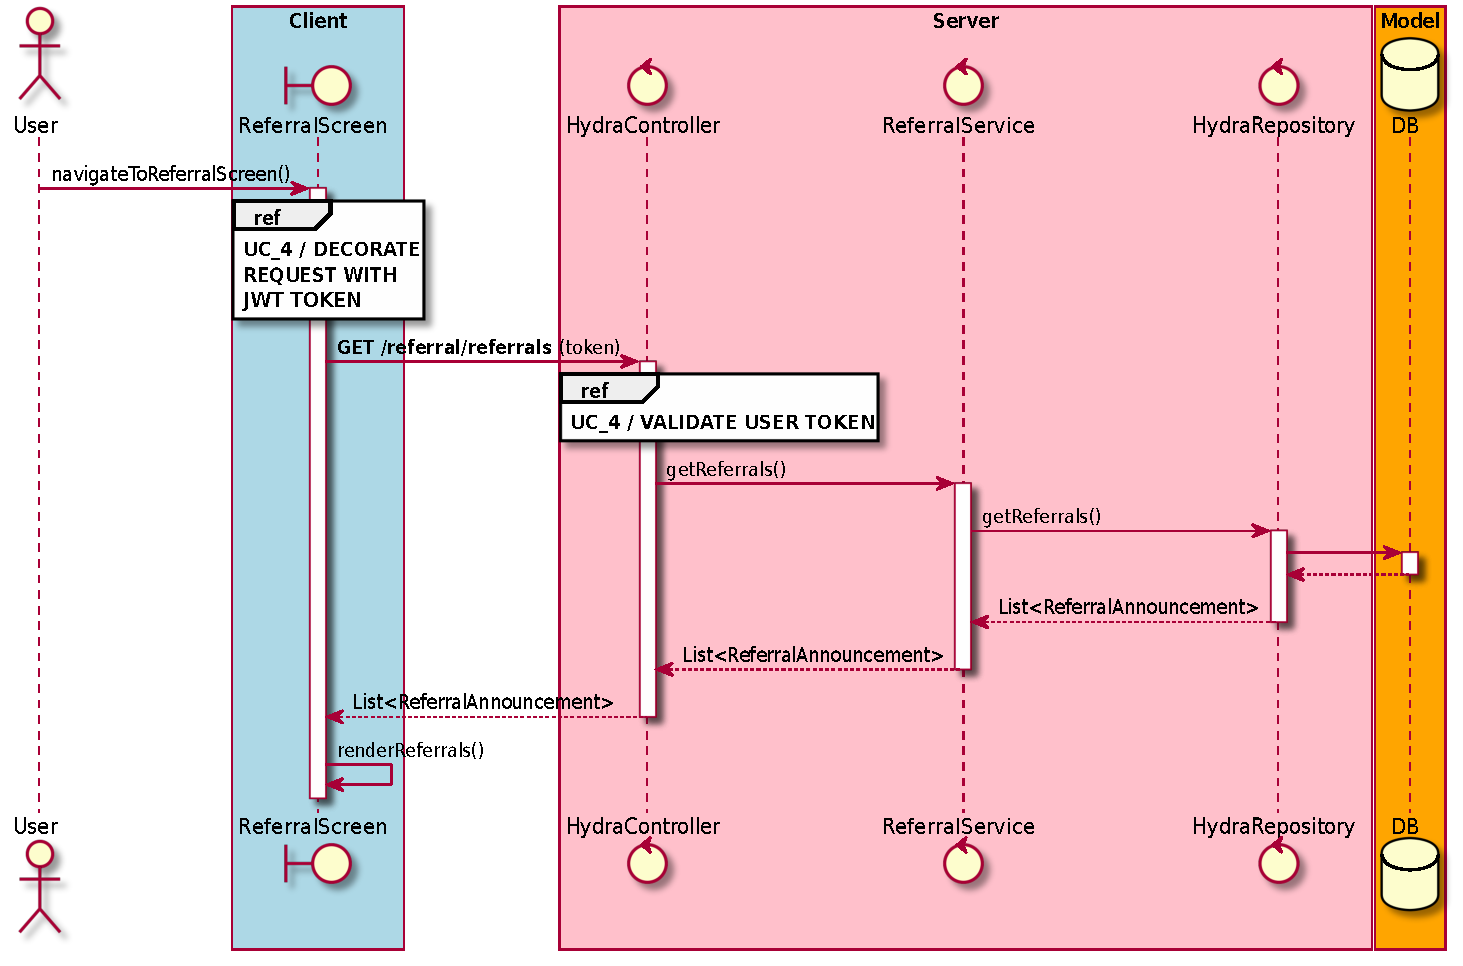
\includegraphics[width=\textwidth, keepaspectratio]{graphics/sequence_diagram_referral_list.pdf}

\section{UC\_11 Wyświetl szczegóły RA}
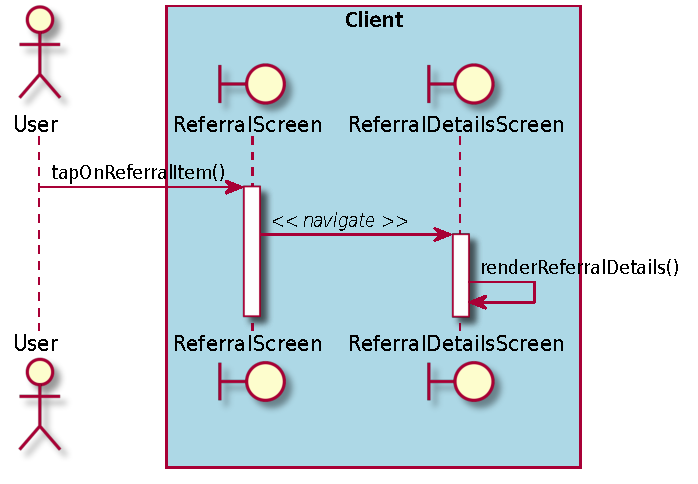
\includegraphics[width=\textwidth, keepaspectratio]{graphics/sequence_diagram_referral_details.pdf}

\chapter{Projekt interfejsu użytkownika IRS}

\section{Ekrany zorientowane wokół Wiki}
\begin{center}
	\makebox[\textwidth]{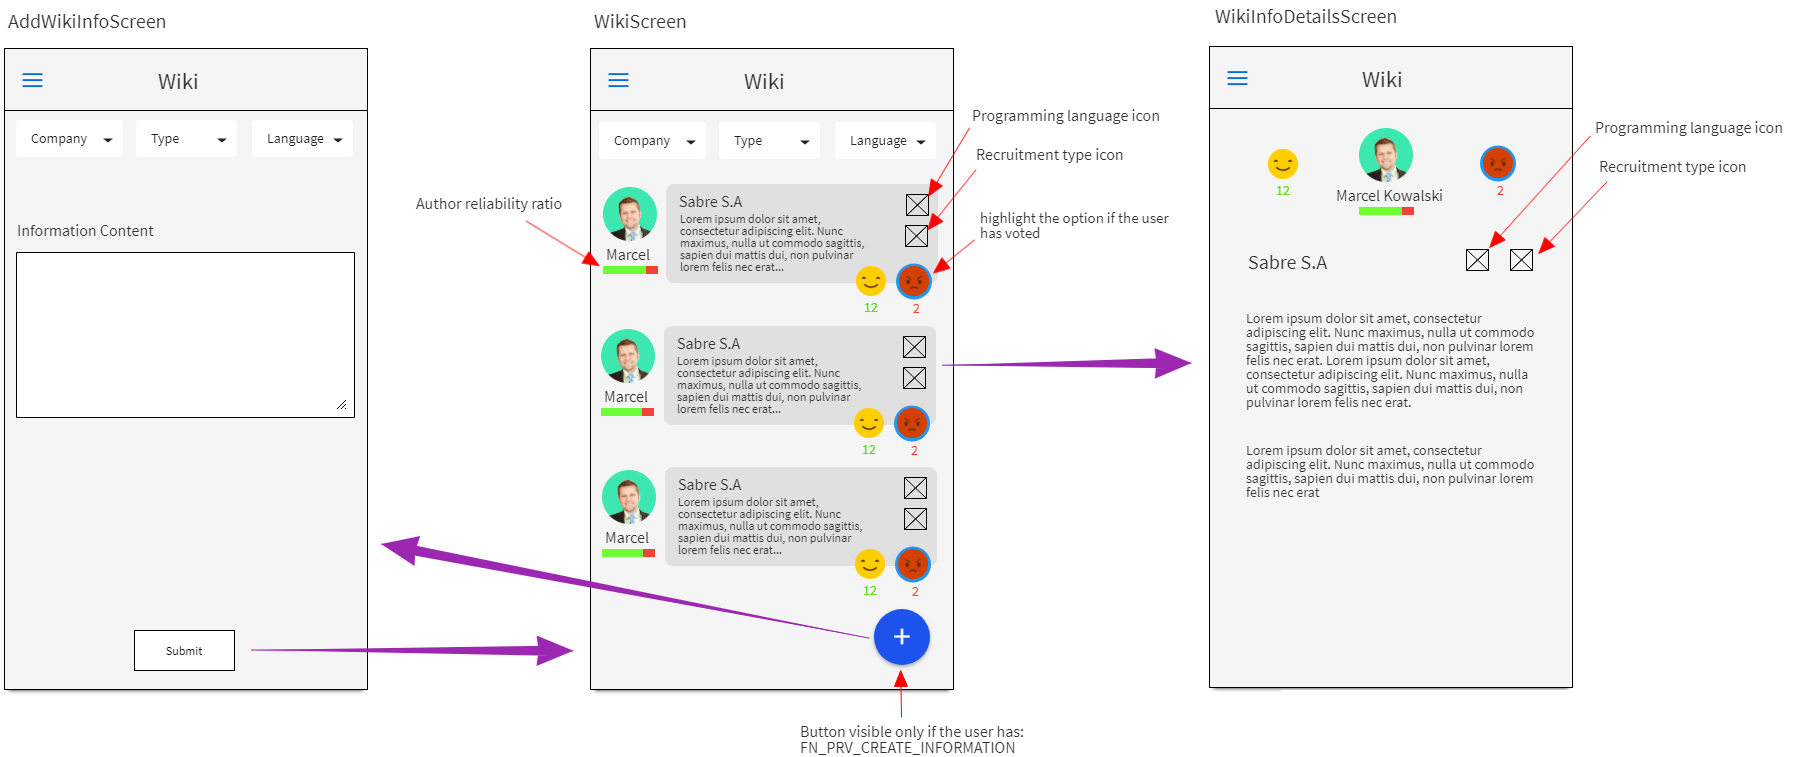
\includegraphics[width=\textwidth]{graphics/wiki_user_interface}}
\end{center}

\section{Ekrany zorientowane wokół Job i Referral}
\begin{center}
	\makebox[\textwidth]{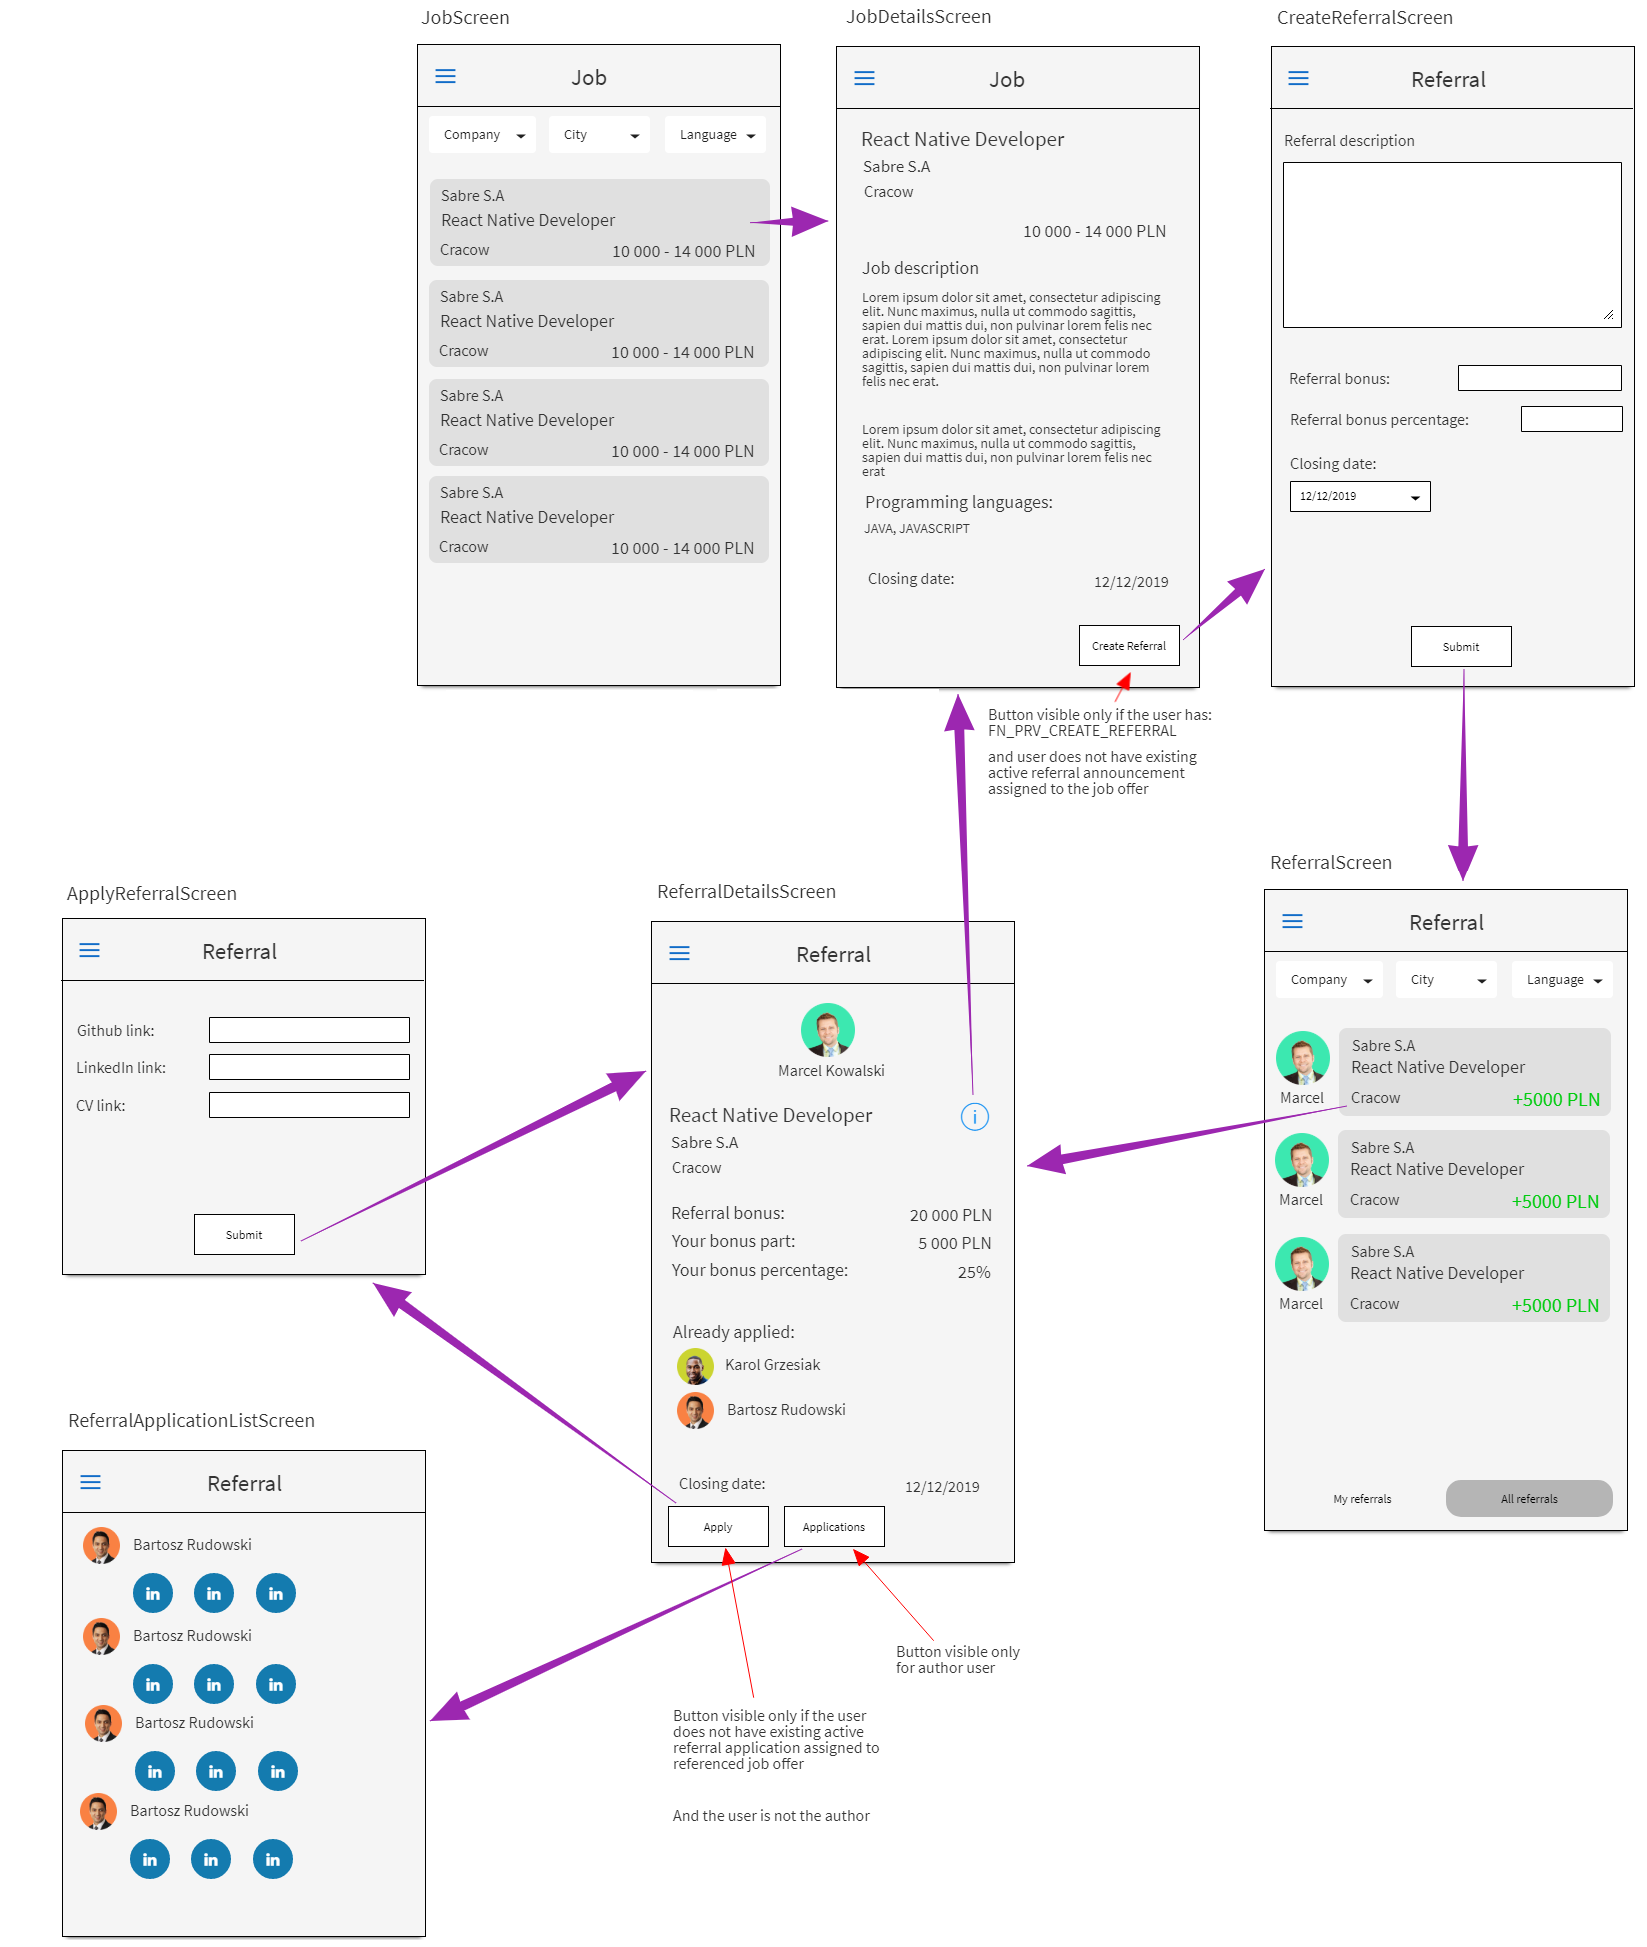
\includegraphics[width=\textwidth]{graphics/job_referral_user_interface}}
\end{center}

\chapter{Projekt bazy danych}

\section{Diagram ERD}
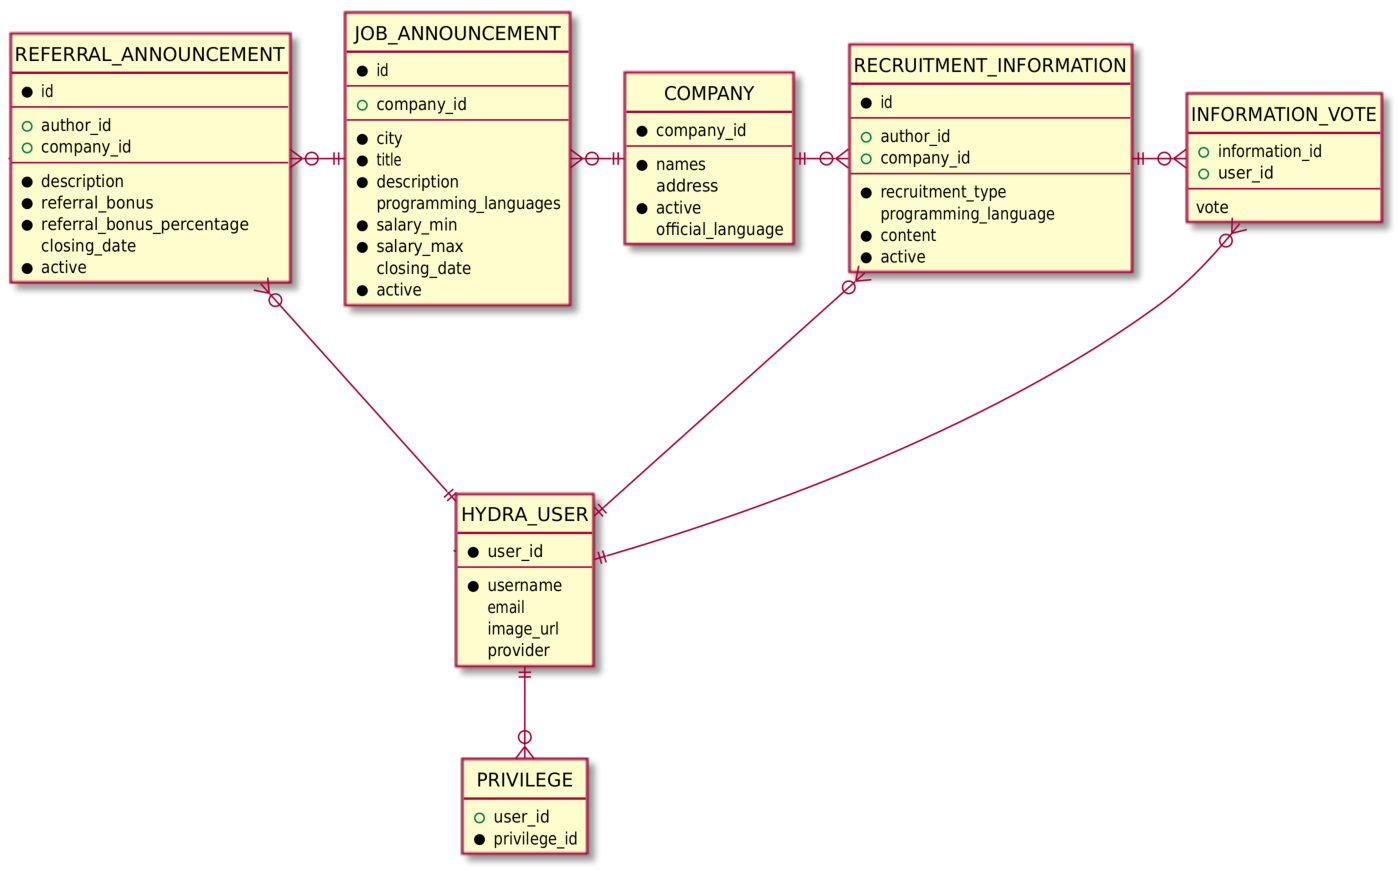
\includegraphics[width=\textwidth, keepaspectratio]{graphics/hydra_db_erd.pdf}

\clearpage
\section{Specyfikacja kwerend}
\begin{table}[ht]
	\centering
	\begin{tabular}{p{4.5cm}|p{5cm}|p{7cm}}
		\textbf{Kwerenda} & \textbf{Zwracana wartość} & \textbf{Opis} \\ \hline
		userExists(userId) & boolean & sprawdza czy dane użytkownika o podanym ID istnieją już w tabeli HYDRA\_USER \\ \hline
		createUser(user) &  & tworzy nowy wiersz w HYDRA\_USER z danymi użytkownika \\ \hline
		getWikiEntries() & List\textless{}Information\textgreater{} & wyciąga z RECRUITMENT\_INFORMATION wszystkie aktywne wpisy \\ \hline
		getUserPrivileges(userId) & List\textless{}Privilege\textgreater{} & wyciąga z tabeli PRIVILEGE uprawnienia przypisane użytkownikowi \\ \hline
		getCompanies() & List\textless{}Company\textgreater{} & wyciąga z tabeli COMPANY wszystkie aktywne informacje o firmach \\ \hline
		addWikiInfo(information) &  & dodaje do tabeli RECRUITMENT\_INFORMATION nowy wpis wiki \\ \hline
		voteForWikiInfo(vote) &  & dodaje lub aktualizuje wpis w tabeli INFORMATION\_VOTE \\ \hline
		getJobs() & List\textless{}JobAnnouncement\textgreater{} & wyciąga z tabeli JOB\_ANNOUNCEMENT wszystkie aktywne oferty pracy, których data ważności wyprzedza aktualną datę \\ \hline
		activeReferralExist(userId, jobId) & boolean & sprawdza czy w tabeli REFERRAL\_ANNOUNCEMENT istnieje aktywna, nieprzeterminowana RA, utworzona przez użytkownika \\ \hline
		addReferral(referral) &  & dodaje do tabeli REFERRAL\_ANNOUNCEMENT nowy wierz z RA \\ \hline
		getReferrals() & List\textless{}ReferralAnnouncement\textgreater{} & wyciąga z tabeli REFERRAL\_ANNOUNCEMENT wszystkie aktywne RA, których data ważności wyprzedza aktualną datę
	\end{tabular}
\end{table}

\end{document}